%%%%%%%% ICML 2024 EXAMPLE LATEX SUBMISSION FILE %%%%%%%%%%%%%%%%%

\documentclass{article}

% Recommended, but optional, packages for figures and better typesetting:
\usepackage{microtype}
\usepackage{graphicx}
\usepackage{subfigure}
\usepackage{booktabs} % for professional tables

% hyperref makes hyperlinks in the resulting PDF.
% If your build breaks (sometimes temporarily if a hyperlink spans a page)
% please comment out the following usepackage line and replace
% \usepackage{icml2024} with \usepackage[nohyperref]{icml2024} above.
\usepackage{hyperref}


% Attempt to make hyperref and algorithmic work together better:
\newcommand{\theHalgorithm}{\arabic{algorithm}}

% Use the following line for the initial blind version submitted for review:
\usepackage{icml2024}

% If accepted, instead use the following line for the camera-ready submission:
% \usepackage[accepted]{icml2024}

% For theorems and such
\usepackage{amsmath}
\usepackage{amssymb}
\usepackage{mathtools}
\usepackage{amsthm}

% if you use cleveref..
% \usepackage[capitalize,noabbrev,nameinlink]{cleveref}
\usepackage[capitalize,nameinlink]{cleveref}

%%%%%%%%%%%%%%%%%%%%%%%%%%%%%%%%
% THEOREMS
%%%%%%%%%%%%%%%%%%%%%%%%%%%%%%%%
\theoremstyle{plain}
\newtheorem{theorem}{Theorem}[section]
\newtheorem{proposition}[theorem]{Proposition}
\newtheorem{lemma}[theorem]{Lemma}
\newtheorem{corollary}[theorem]{Corollary}
\theoremstyle{definition}
\newtheorem{definition}[theorem]{Definition}
\newtheorem{assumption}[theorem]{Assumption}
\theoremstyle{remark}
\newtheorem{remark}[theorem]{Remark}

% Todonotes is useful during development; simply uncomment the next line
%    and comment out the line below the next line to turn off comments
%\usepackage[disable,textsize=tiny]{todonotes}
\usepackage[textsize=tiny]{todonotes}


% The \icmltitle you define below is probably too long as a header.
% Therefore, a short form for the running title is supplied here:
\icmltitlerunning{Sample-Efficient RL with Implicitly Quantized Representations}

%%%%%%%%%%%%%%%%%%%%%%%%%%%%%%%%
% CUSTOM (our stuff)
%%%%%%%%%%%%%%%%%%%%%%%%%%%%%%%%

% \newcommand{\our}{\textsc{vq-td3}\xspace}
% \newcommand{\our}{\textsc{iFSQ-RL}\xspace}
\newcommand{\ourrew}{\textsc{iQRL+rew}\xspace}
\newcommand{\ourcosrew}{\textsc{iQRL+cos+rew}\xspace}
\newcommand{\our}{\textsc{iQRL}\xspace}

% Latin
\usepackage{xspace}
\newcommand{\eg}{\textit{e.g.\@}\xspace}
\newcommand{\ie}{\textit{i.e.\@}\xspace}
\newcommand{\cf}{\textit{cf.\@}\xspace}
\newcommand{\etc}{\textit{etc.\@}\xspace}
\newcommand{\etal}{\textit{et~al.\@}\xspace}

% Vectors
\usepackage{bm}
\def\vzero{{\bm{0}}}
\def\vone{{\bm{1}}}
\def\vmu{{\bm{\mu}}}
\def\vtheta{{\bm{\theta}}}
\def\va{{\bm{a}}}
\def\vb{{\bm{b}}}
\def\vc{{\bm{c}}}
\def\vd{{\bm{d}}}
\def\ve{{\bm{e}}}
\def\vf{{\bm{f}}}
\def\vg{{\bm{g}}}
\def\vh{{\bm{h}}}
\def\vi{{\bm{i}}}
\def\vj{{\bm{j}}}
\def\vk{{\bm{k}}}
\def\vl{{\bm{l}}}
\def\vm{{\bm{m}}}
\def\vn{{\bm{n}}}
\def\vo{{\bm{o}}}
\def\vp{{\bm{p}}}
\def\vq{{\bm{q}}}
\def\vr{{\bm{r}}}
\def\vs{{\bm{s}}}
\def\vt{{\bm{t}}}
\def\vu{{\bm{u}}}
\def\vv{{\bm{v}}}
\def\vw{{\bm{w}}}
\def\vx{{\bm{x}}}
\def\vy{{\bm{y}}}
\def\vz{{\bm{z}}}

% Elements of vectors
\def\evalpha{{\alpha}}
\def\evbeta{{\beta}}
\def\evepsilon{{\epsilon}}
\def\evlambda{{\lambda}}
\def\evomega{{\omega}}
\def\evmu{{\mu}}
\def\evpsi{{\psi}}
\def\evsigma{{\sigma}}
\def\evtheta{{\theta}}
\def\eva{{a}}
\def\evb{{b}}
\def\evc{{c}}
\def\evd{{d}}
\def\eve{{e}}
\def\evf{{f}}
\def\evg{{g}}
\def\evh{{h}}
\def\evi{{i}}
\def\evj{{j}}
\def\evk{{k}}
\def\evl{{l}}
\def\evm{{m}}
\def\evn{{n}}
\def\evo{{o}}
\def\evp{{p}}
\def\evq{{q}}
\def\evr{{r}}
\def\evs{{s}}
\def\evt{{t}}
\def\evu{{u}}
\def\evv{{v}}
\def\evw{{w}}
\def\evx{{x}}
\def\evy{{y}}
\def\evz{{z}}

% Matrix
\def\mA{{\bm{A}}}
\def\mB{{\bm{B}}}
\def\mC{{\bm{C}}}
\def\mD{{\bm{D}}}
\def\mE{{\bm{E}}}
\def\mF{{\bm{F}}}
\def\mG{{\bm{G}}}
\def\mH{{\bm{H}}}
\def\mI{{\bm{I}}}
\def\mJ{{\bm{J}}}
\def\mK{{\bm{K}}}
\def\mL{{\bm{L}}}
\def\mM{{\bm{M}}}
\def\mN{{\bm{N}}}
\def\mO{{\bm{O}}}
\def\mP{{\bm{P}}}
\def\mQ{{\bm{Q}}}
\def\mR{{\bm{R}}}
\def\mS{{\bm{S}}}
\def\mT{{\bm{T}}}
\def\mU{{\bm{U}}}
\def\mV{{\bm{V}}}
\def\mW{{\bm{W}}}
\def\mX{{\bm{X}}}
\def\mY{{\bm{Y}}}
\def\mZ{{\bm{Z}}}
\def\mBeta{{\bm{\beta}}}
\def\mPhi{{\bm{\Phi}}}
\def\mLambda{{\bm{\Lambda}}}
\def\mSigma{{\bm{\Sigma}}}

\newcommand{\E}{\mathbb{E}}
\newcommand{\Ls}{\mathcal{L}}
\newcommand{\R}{\mathbb{R}}
\newcommand{\emp}{\tilde{p}}
\newcommand{\lr}{\alpha}
\newcommand{\reg}{\lambda}
\newcommand{\rect}{\mathrm{rectifier}}
\newcommand{\softmax}{\mathrm{softmax}}
\newcommand{\sigmoid}{\sigma}
\newcommand{\softplus}{\zeta}
\newcommand{\KL}{D_{\mathrm{KL}}}
\newcommand{\Var}{\mathrm{Var}}
\newcommand{\standarderror}{\mathrm{SE}}
\newcommand{\Cov}{\mathrm{Cov}}
% Wolfram Mathworld says $L^2$ is for function spaces and $\ell^2$ is for vectors
% But then they seem to use $L^2$ for vectors throughout the site, and so does
% wikipedia.
\newcommand{\normlzero}{L^0}
\newcommand{\normlone}{L^1}
\newcommand{\normltwo}{L^2}
\newcommand{\normlp}{L^p}
\newcommand{\normmax}{L^\infty}

\DeclareMathOperator*{\argmax}{arg\,max}
\DeclareMathOperator*{\argmin}{arg\,min}

\usetikzlibrary{shapes.geometric,positioning,calc}

% Arno's cube hack
\newcommand{\cube}{%
\resizebox{1em}{.9em}{
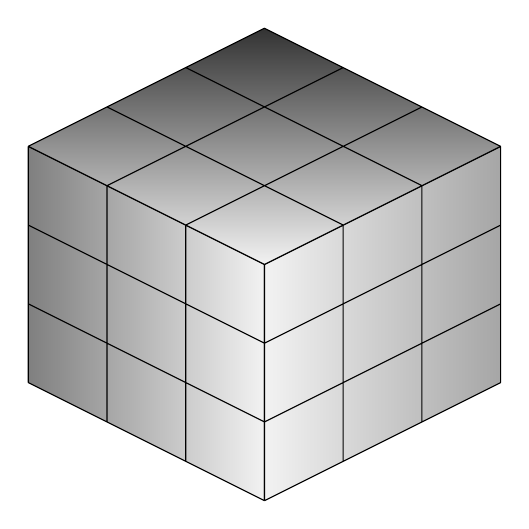
\begin{tikzpicture}[baseline=-1ex,cube/.style={very thick,black},
            grid/.style={very thin,gray},
            axis/.style={->,black,thick}]
 \begin{scope}[every node/.append style={yslant=-0.5},yslant=-0.5]
 [cube/.style={very thick,black},
            axis/.style={->,blue,thick}]
   \shade[right color=gray!10, left color=black!50] (0,0) rectangle +(3,3);
   \node at (0.5,2.5) {};
   \node at (1.5,2.5) {};
   \node at (2.5,2.5) {};
   \node at (0.5,1.5) {};
   \node at (1.5,1.5) {};
   \node at (2.5,1.5) {};
   \node at (0.5,0.5) {};
   \node at (1.5,0.5) {};
   \node at (2.5,0.5) {};
   \draw (0,0) grid (3,3);
 \end{scope}
 
 \begin{scope}[every node/.append style={yslant=0.5},yslant=0.5]
   \shade[right color=gray!70,left color=gray!10] (3,-3) rectangle +(3,3);
   \node at (3.5,-0.5) {};
   \node at (4.5,-0.5) {};
   \node at (5.5,-0.5) {};
   \node at (3.5,-1.5) {};
   \node at (4.5,-1.5) {};
   \node at (5.5,-1.5) {};
   \node at (3.5,-2.5) {};
   \node at (4.5,-2.5) {};
   \node at (5.5,-2.5) {};
   \draw (3,-3) grid (6,0);
 \end{scope}

 \begin{scope}[every node/.append style={
     yslant=0.5,xslant=-1},yslant=0.5,xslant=-1
   ]
   \shade[bottom color=gray!10, top color=black!80] (6,3) rectangle +(-3,-3);
   \node at (3.5,2.5) {};
   \node at (3.5,1.5) {};
   \node at (3.5,0.5) {};
   \node at (4.5,2.5) {};
   \node at (4.5,1.5) {};
   \node at (4.5,0.5) {};
   \node at (5.5,2.5) {};
   \node at (5.5,1.5) {};
   \node at (5.5,0.5) {};
   \draw (3,0) grid (6,3);  
 \end{scope}
\end{tikzpicture}}}


%%%%%%%%%%%%%%%%%%%%%%%%%%%%%%%%
% BEGIN DOCUMENT
%%%%%%%%%%%%%%%%%%%%%%%%%%%%%%%%
\begin{document}

\twocolumn[
% \icmltitle{Submission and Formatting Instructions for \\
%            International Conference on Machine Learning (ICML 2024)}
% \icmltitle{Sample-efficient Reinforcement Learning with Latent Representations}
\icmltitle{Sample-Efficient Reinforcement Learning \\ with Implicitly Quantized Representations}

% It is OKAY to include author information, even for blind
% submissions: the style file will automatically remove it for you
% unless you've provided the [accepted] option to the icml2024
% package.

% List of affiliations: The first argument should be a (short)
% identifier you will use later to specify author affiliations
% Academic affiliations should list Department, University, City, Region, Country
% Industry affiliations should list Company, City, Region, Country

% You can specify symbols, otherwise they are numbered in order.
% Ideally, you should not use this facility. Affiliations will be numbered
% in order of appearance and this is the preferred way.
\icmlsetsymbol{equal}{*}

\begin{icmlauthorlist}
\icmlauthor{Aidan Scannell}{aalto,fcai}
\icmlauthor{Kalle Kujanpää}{aalto,fcai}
\icmlauthor{Yi Zhao}{aalto}
\icmlauthor{Arno Solin}{aalto}
\icmlauthor{Joni Pajarinen}{aalto}
% \icmlauthor{Firstname1 Lastname1}{equal,yyy}
% \icmlauthor{Firstname2 Lastname2}{equal,yyy,comp}
% \icmlauthor{Firstname3 Lastname3}{comp}
% \icmlauthor{Firstname4 Lastname4}{sch}
% \icmlauthor{Firstname5 Lastname5}{yyy}
% \icmlauthor{Firstname6 Lastname6}{sch,yyy,comp}
% \icmlauthor{Firstname7 Lastname7}{comp}
% %\icmlauthor{}{sch}
% \icmlauthor{Firstname8 Lastname8}{sch}
% \icmlauthor{Firstname8 Lastname8}{yyy,comp}
%\icmlauthor{}{sch}
%\icmlauthor{}{sch}
\end{icmlauthorlist}

\icmlaffiliation{aalto}{Aalto University, Finland}
\icmlaffiliation{fcai}{Finnish Center for Artificial Intelligence}
% \icmlaffiliation{yyy}{Department of XXX, University of YYY, Location, Country}
% \icmlaffiliation{comp}{Company Name, Location, Country}
% \icmlaffiliation{sch}{School of ZZZ, Institute of WWW, Location, Country}

\icmlcorrespondingauthor{Aidan Scannell}{aidan.scannell@aalto.fi}
% \icmlcorrespondingauthor{Firstname1 Lastname1}{first1.last1@xxx.edu}
% \icmlcorrespondingauthor{Firstname2 Lastname2}{first2.last2@www.uk}

% You may provide any keywords that you
% find helpful for describing your paper; these are used to populate
% the "keywords" metadata in the PDF but will not be shown in the document
\icmlkeywords{Machine Learning, ICML}

\vskip 0.3in
]

% this must go after the closing bracket ] following \twocolumn[ ...

% This command actually creates the footnote in the first column
% listing the affiliations and the copyright notice.
% The command takes one argument, which is text to display at the start of the footnote.
% The \icmlEqualContribution command is standard text for equal contribution.
% Remove it (just {}) if you do not need this facility.

\printAffiliationsAndNotice{}  % leave blank if no need to mention equal contribution
% \printAffiliationsAndNotice{\icmlEqualContribution} % otherwise use the standard text.


\begin{abstract}
  Learning representations for reinforcement learning (RL) has shown much promise for continuous control. We propose an efficient representation learning method using only a self-supervised latent-state consistency loss. Our approach employs an encoder and a dynamics model to map observations to latent states and predict future states, respectively. We achieve high performance and prevent representation collapse by normalizing and bounding the latent representation such that rank in the representation is empirically preserved. Our method is straightforward, compatible with any model-free RL algorithm, and demonstrates state-of-the-art performance in continuous control benchmarks from DeepMind Control Suite.
\end{abstract}

% \begin{abstract}
%   In reinforcement learning (RL) for continuous control, we propose an
%   efficient representation learning method using only a latent-state
%   consistency loss. Our approach employs an encoder and a transition
%   model to map observations to latent states and predict future
%   states, respectively. We achieve high performance and prevent
%   representation collapse by normalizing the quantized latent
%   representation such that rank in the presentation is empirically
%   preserved. Our method is straightforward, compatible with any
%   model-free RL algorithm, and demonstrates state-of-the-art
%   performance in continuous control benchmarks from DeepMind Control
%   Suite.
% \end{abstract}

%% \begin{abstract}
%%   Learning representations for reinforcement learning (RL) has shown
%%   much promise for continuous control. Representations not only can
%%   handle complex observation spaces but also improve sample
%%   efficiency. A particularly promising approach is to use a
%%   self-supervised latent-state consistency loss with observation to
%%   latent state mapping, together with next latent state, reward, and
%%   value predictions. Reward and value predictions prevent
%%   representation collapse at the cost of learning a task-specific
%%   representation.  We show how to use only the latent-state
%%   consistency loss to {\em (i)} learn a task-agnostic representation
%%   and {\em (ii)} prevent representation collapse by normalizing and
%%   bounding the latent representation. In experiments, our approach
%%   which be combined with any model-free RL algorithm obtains
%%   state-of-the-art results in continuous control benchmarks from
%%   DeepMind Control Suite.
%% \end{abstract}

%% \begin{abstract}
%%   % Deep reinforcement learning (RL) has shown much promise for solving real-world continuous control problems.
%%   % Whilst deep reinforcement learning (RL) is a competitive approach for solving real-world continuous control problems, it
%%   % is limited by its sample-efficiency.
%%   % Recent works have shown that learning representations can improve sample efficiency in RL, whilst also
%%   % handling complex/high-dimensional observation spaces.
%%   Learning representations for reinforcement learning (RL) has shown much promise for continuous control.
%%   Not only can it handle complex observation spaces but it can also improve sample efficiency.
%%   % Recent works have shown that learning representations can improve sample efficiency in RL.
%%   A particularly promising approach is to use a self-supervised loss, known as the latent-state consistency loss.
%%   It requires an encoder which maps observations to latent states and a transition model which predicts
%%   next latent states.
%%   It then minimizes the distance between the next state predicted by the transition model and
%%   the next state predicted by the encoder.
%%   Typically it is combined with other loss terms such as reward or value prediction.
%%   This prevents representation collapse at the cost of learning a task-specific representation.
%%   In this work, we show that a careful consideration of the latent space enables us to {\em (i)} learn
%%   a task-agnostic representation and {\em (ii)} prevent representation collapse, whilst using only the latent-state
%%   consistency loss.
%%   % the leverage the latent-state
%%   % Typically these approaches have unbounded latent spaces and are combined with auxillary loss terms such as minimizing the
%%   % error of reward or value predictions in the latent space.
%%   % of an encoder which maps observations to latent states and a transition model which predicts
%%   % next latent states given a latent state and an action.
%%   % However, most of th
%%   We empirically show that our method prevents representation collapse as it maintains matrix rank.
%%   Our representation learning approach is {\em (i)} simple, {\em (ii)} can be combined with any model-free RL algorithm
%%   and, {\em (iii)} obtains state-of-the-art results in continuous control benchmarks from DeepMind Control Suite.
%%   % Moreover, it kk
%% % This document provides a basic paper template and submission guidelines.
%% % Abstracts must be a single paragraph, ideally between 4--6 sentences long.
%% % Gross violations will trigger corrections at the camera-ready phase.
%% \end{abstract}


% \section{Introduction}
% \label{intro}

% Reinforcement learning (RL) \citep{sutton2018reinforcement} has shown much promise in games, animation and robotics.
% However, applying RL in real-world environments is challenging. The problem is two-fold,
% {\em (i)}, handling high dimensional/complex observation spaces is non-trivial and {\em (ii)}
% deep RL typically requires millions of data points which can be unpractical (or costly), \ie it is very sample inefficient.

% % Given such a latent space,
% % Whilst these latent states are often lower dimensional this is not always
% Many approaches have been proposed to improve sample efficiency in deep RL.
% As \citet{laskinCURLContrastiveUnsupervised2020} highlighted, these can generally be divided into two streams of research:
% {\em (i)} auxillary tasks on the agent's observations and {\em (ii)} world models that predict the future
% \citep{haRecurrentWorldModels2018,hafnerLearning2019,hansenTemporalDifferenceLearning2022}.
% In this work, we are interested in the first class of methods, which use auxillary tasks to improve sample efficiency.
% In particular, methods for compressing observations into latent states.%, aka representation learning.

% Learning representations for RL has been investigated for decades
% \citep{abelOptimalBehaviorApproximate2016,mannorDynamicAbstractionReinforcement2004,liUnifiedTheoryState2006,andreStateAbstractionProgrammable2002,deardenAbstractionApproximateDecisiontheoretic1997,singhReinforcementLearningSoft1994,higginsDefinitionDisentangledRepresentations2018,vanhoofStableReinforcementLearning2016,watterEmbedControlLocally2015,ghoshRepresentationsStableOffPolicy2020}.
% However, these approaches are usually limited to simple environments.
% Some approaches used unsupervised learning (\eg VAE \citep{kingmaAutoEncoding2014} with reconstruction loss) to acquire representations
% \citep{finnDeepSpatialAutoencoders2016,higginsDARLAImprovingZeroShot2017,langeAutonomousReinforcementLearning2012,watterEmbedControlLocally2015}.
% More recently, self-supervised learning (SSL) approaches (which do not reconstruct observations)
% attempt to learn good features without labels \cite{anandUnsupervisedStateRepresentation2019}.
% Alternative approaches leverage contrastive losses to learn representations \cite{laskinCURLContrastiveUnsupervised2020}.

\begin{figure}[t!]
\centering\scriptsize
%\resizebox{\columnwidth}{!}{%
%\begin{tikzpicture}
%
%  % Declare that we have a background layer (advanced)
%  \pgfdeclarelayer{background}
%  \pgfsetlayers{background,main}
%
%  % Helpers for small subscripts
%  \newcommand{\sub}[0]{\scalebox{.8}{\ensuremath t}}
%  \newcommand{\subs}[1]{\scalebox{.8}{\ensuremath t{+}#1}}
%
%  % Lengths (this tunes distance)
%  \newlength{\nodedist}\setlength{\nodedist}{2cm}
%
%  % Styles (this tunes colours etc.)
%  \tikzstyle{mynode}=[fill=blue!10!cyan,rounded corners=1pt,font=\tiny,inner sep=0]
%  \tikzstyle{trap}=[mynode,trapezium,minimum width=1.5em, minimum height=2em,
%                    trapezium left angle=-70, trapezium right angle=-70]
%  \tikzstyle{blob}=[mynode,circle,minimum width=2.4em,minimum height=2.4em]
%  \tikzstyle{polval}=[mynode,minimum width=6em,minimum height=2em,align=center,text=white,fill=black!60,inner sep=2pt]
%  \tikzstyle{arr}=[line width=1pt,black,->]
%  \tikzstyle{darr}=[line width=1pt,black,<->,densely dotted]
%
%  % *** FIRST HALF ***
%
%  % Draw nodes
%  \node[blob] (z0) at (0\nodedist,0) {$\vz_{\sub}$};
%  \node[blob] (z1) at (1\nodedist,0) {$\hat\vz_{\subs{1}}$};
%  \node[blob] (z2) at (2\nodedist,0) {$\hat\vz_{\subs{2}}$};
%
%  \node[trap] (e0) at (0\nodedist,\nodedist) {$e_\phi$};
%  \node[trap] (e1) at (1\nodedist,\nodedist) {$e_{\bar\phi}$};
%  \node[trap] (e2) at (2\nodedist,\nodedist) {$e_{\bar\phi}$};
%
%  \node[blob] (zh1) at ($(z1)!0.5!(e1)$) {$\bar\vz_{\subs{1}}$};
%  \node[blob] (zh2) at ($(z2)!0.5!(e2)$) {$\bar\vz_{\subs{2}}$};
%
%  \coordinate (m0) at ($(z0)!.5!(z1)$);
%  \node[blob] (a0) at ($(m0)!(zh1)!(m0)$) {$\va_{\sub}$};
%  \coordinate (m1) at ($(z1)!.5!(z2)$);
%  \node[blob] (a1) at ($(m1)!(zh2)!(m1)$) {$\va_{\subs{1}}$};
%
%  \node[mynode,above of=e0] (i0) {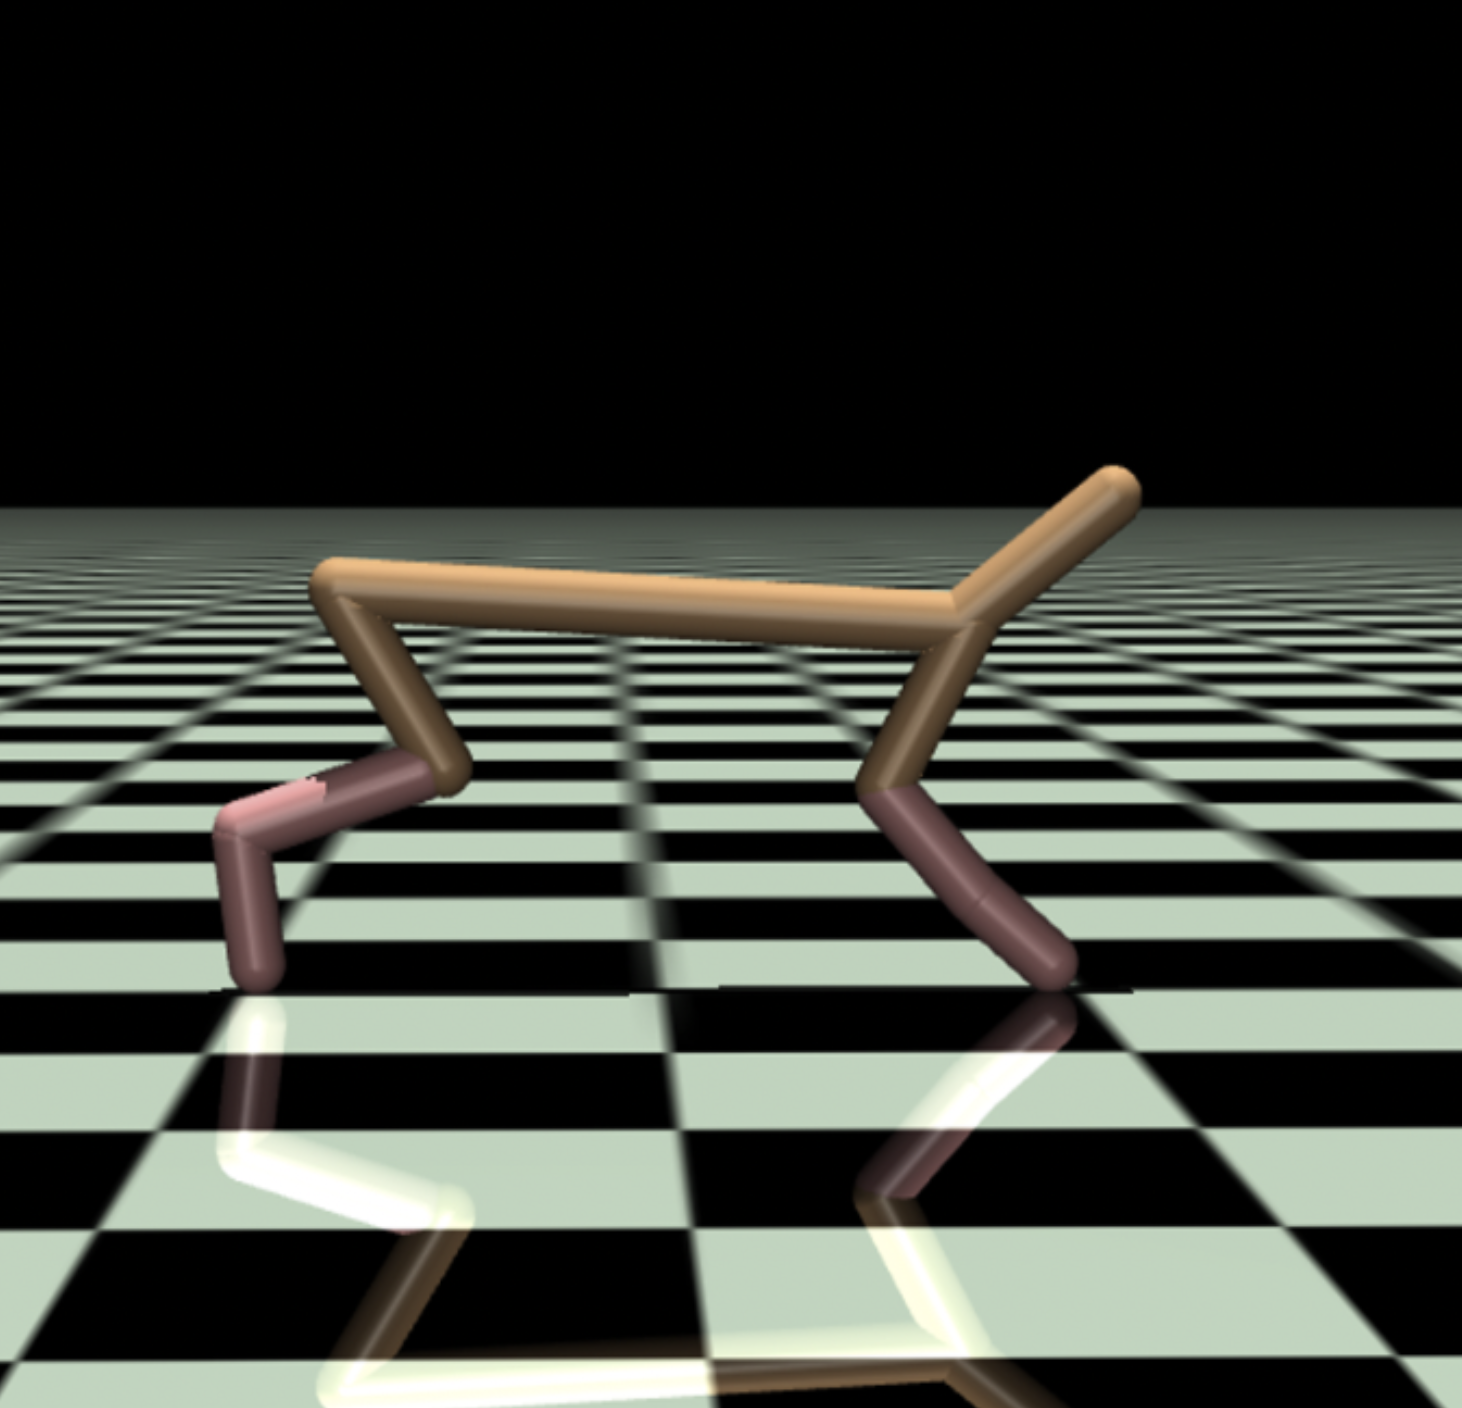
\includegraphics[width=4.7em]{figs/bg}};
%  \node[mynode,above of=e1] (i1) {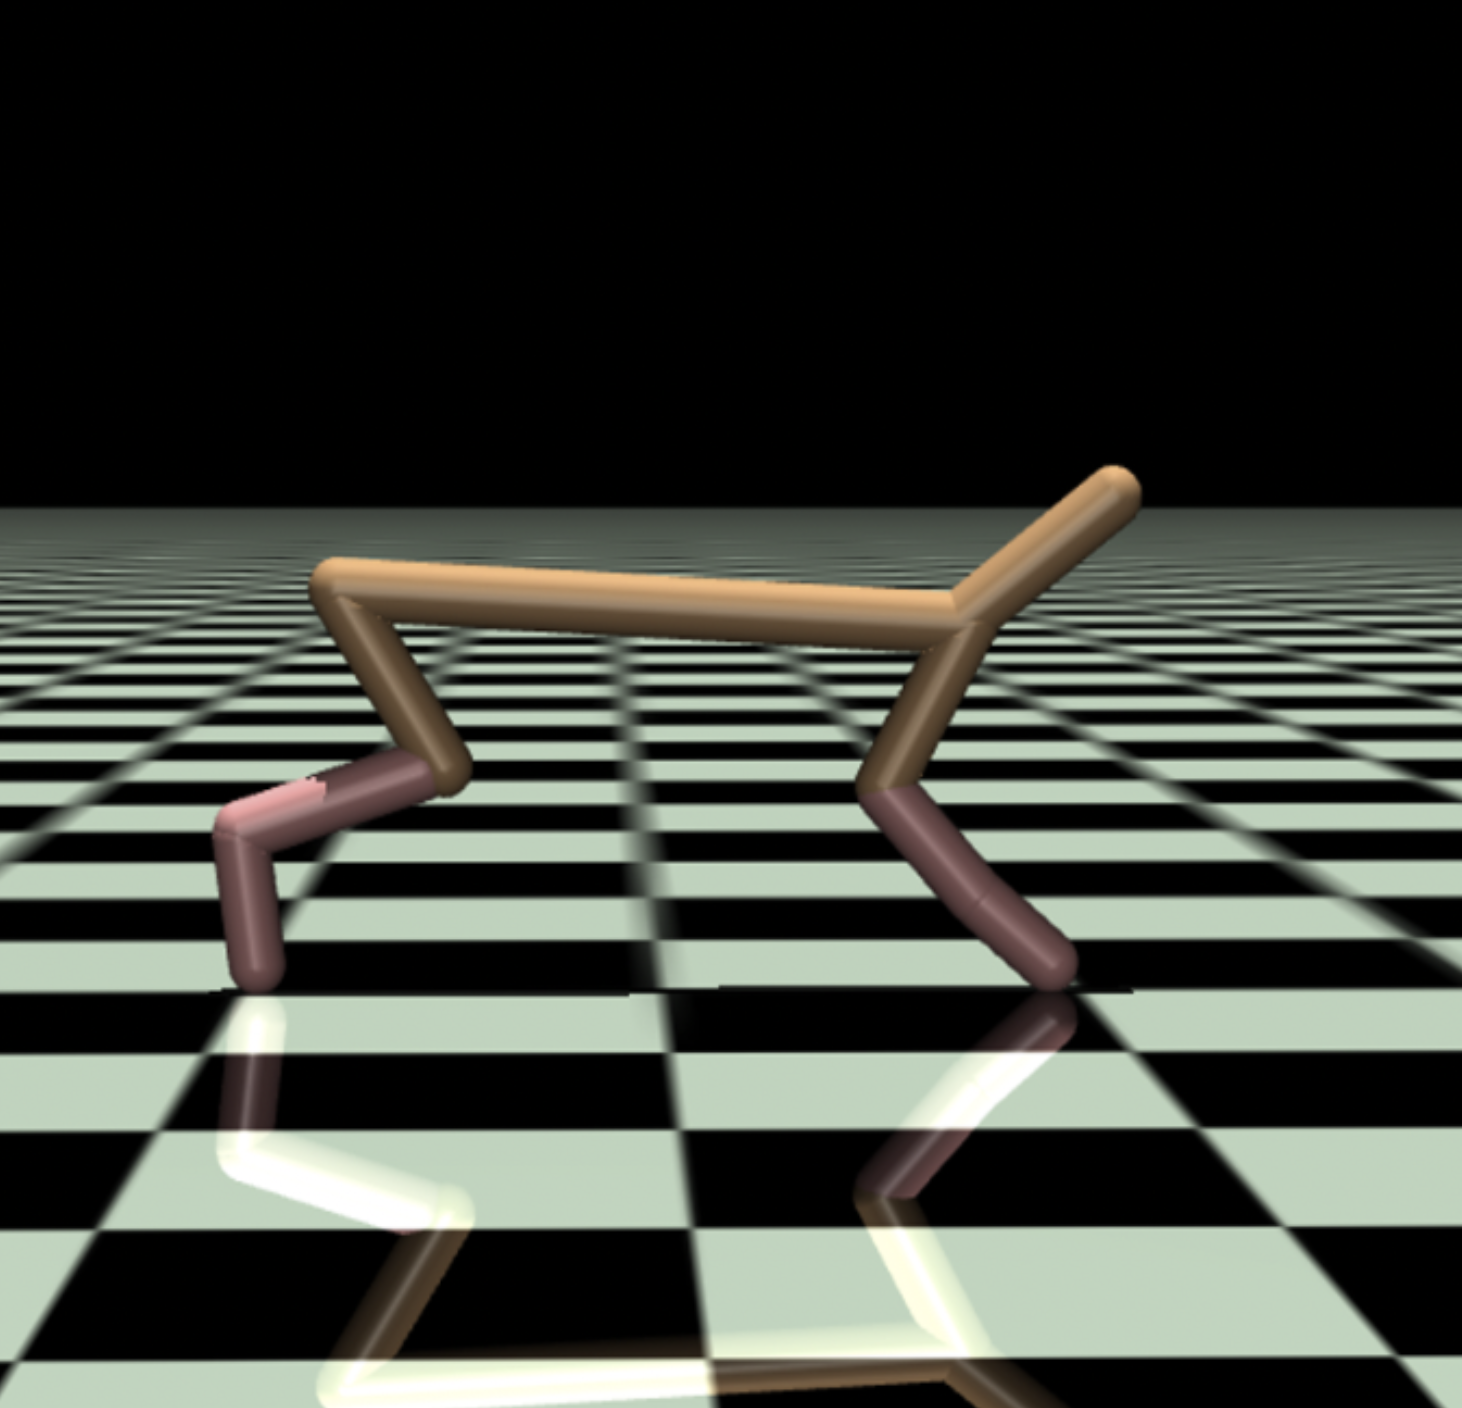
\includegraphics[width=4.7em]{figs/bg}};
%  \node[mynode,above of=e2] (i2) {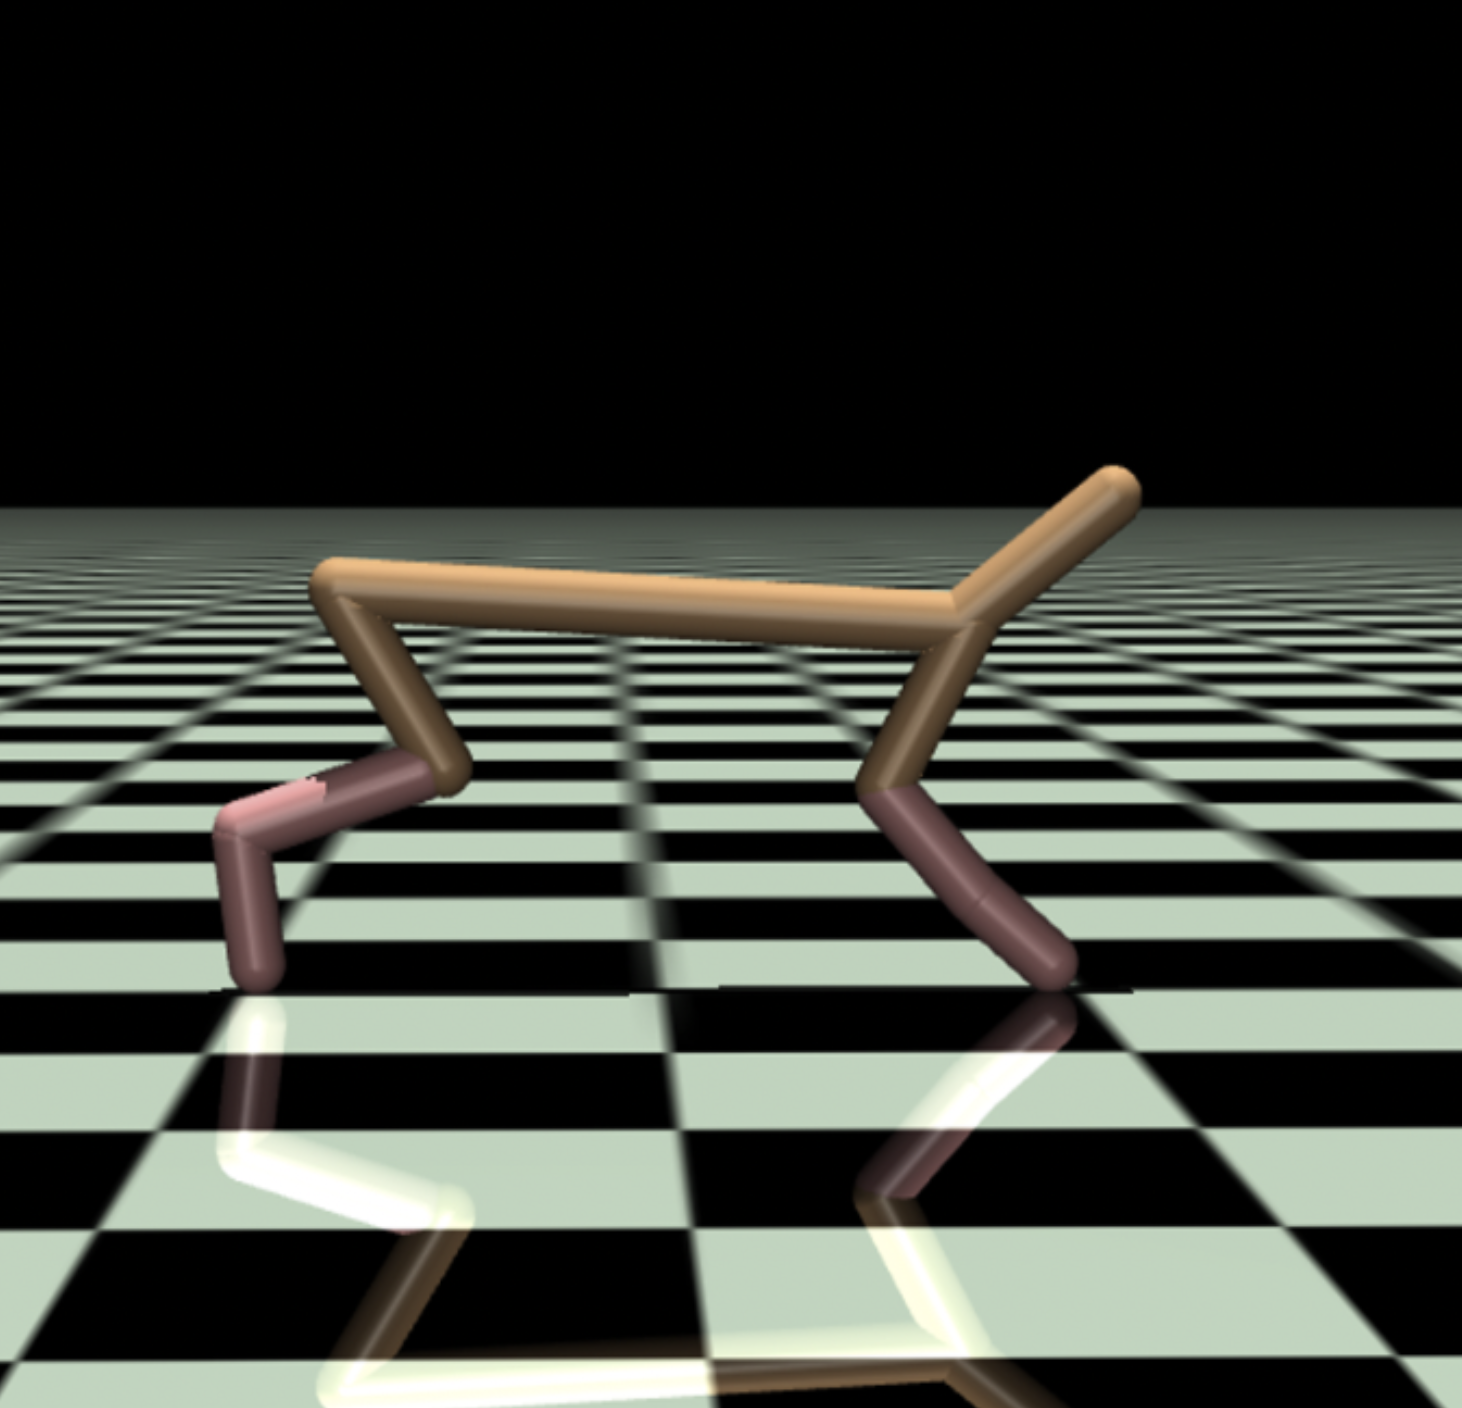
\includegraphics[width=4.7em]{figs/bg}};
%
%  \node[anchor=north] (o0) at (i0.north) {\color{white}$o_{\sub}$};
%  \node[anchor=north] (o1) at (i1.north) {\color{white}$o_{\subs{1}}$};
%  \node[anchor=north] (o2) at (i2.north) {\color{white}$o_{\subs{2}}$};
%
%  \node[above of=i1,align=center] (lab0) {\normalsize\bf 1.\ Learn representation};
%
%  % Draw arrows
%  \draw[arr] (i0) -- (e0);
%  \draw[arr] (i1) -- (e1);
%  \draw[arr] (i2) -- (e2);
%  \draw[arr] (z0) -- (z1);
%  \draw[arr] (z1) -- (z2);
%  \draw[arr] (e0) -- (z0);
%  \draw[arr] (e1) -- (zh1);
%  \draw[arr] (e2) -- (zh2);
%  \draw[arr] (a0) -- (z1);
%  \draw[arr] (a1) -- (z2);
%  \draw[darr] (zh1) -- (z1);
%  \draw[darr] (zh2) -- (z2);
%
%
%  % *** SECOND HALF ***
%
%  \node[blob] (z) at ($(e2) + (1.5\nodedist,0)$) {$\bar\vz_{\sub}$};
%  \node[polval] (policy) at ($(z) + (-.5\nodedist,-.5\nodedist)$) {{\bf Policy} \\ $\pi_\theta(\va_t \mid \bar\vz_t)$};
%  \node[polval] (value) at ($(z) + (.5\nodedist,-.5\nodedist)$) {{\bf Value} \\ $\mathcal{Q}_\psi(\bar\vz_t, \va_t)$};
%
%  \draw[arr] (z) -- (policy);
%  \draw[arr] (z) -- (value);
%
%  \node[align=center] at ($(z)!(lab0)!(z)$) {\normalsize\bf 2.\ Latent actor-critic\vphantom{p}};
%
%  % Draw backgrounds
%  \begin{pgfonlayer}{background}
%
%    \coordinate (mid) at ($(i2.east)!.5!(policy.west)$);
%
%    \draw[draw=none,fill=black!10,rounded corners=5pt] ($(i0.north west) + (-.25cm,1cm)$)
%      rectangle ($(mid)!(z2.north)!(mid) + (-3pt,-1cm)$);
%
%    \draw[draw=none,fill=black!05,rounded corners=5pt] ($(mid)!(i2.north east)!(mid) + (3pt,1cm)$)
%      rectangle ($(value.east)!(z2.north)!(value.east) + (.25cm,-1cm)$);
%
%  \end{pgfonlayer}
%
%\end{tikzpicture}}

\begin{tikzpicture}

  % Declare that we have a background layer (advanced)
  \pgfdeclarelayer{background}
  \pgfsetlayers{background,main}

  % Helpers for small subscripts
  \newcommand{\sub}[0]{\scalebox{.8}{\ensuremath t}}
  \newcommand{\subs}[1]{\scalebox{.8}{\ensuremath t{+}#1}}

  % Lengths (this tunes distance)
  \newlength{\nodedist}\setlength{\nodedist}{3cm}
  \newlength{\nodedistv}\setlength{\nodedistv}{2.5cm}

  % Styles (this tunes colours etc.)
  \tikzstyle{mynode}=[fill=black!5,draw=black!20,rounded corners=1pt,font=\tiny,inner sep=0,align=center,line width=1pt]
  \tikzstyle{trap}=[mynode,trapezium,text width=6.5em, minimum height=2em,
                    trapezium left angle=-70, trapezium right angle=-70,inner sep=2pt]
  \tikzstyle{blob}=[mynode,circle,minimum width=2.4em,minimum height=2.4em]
  \tikzstyle{polval}=[mynode,minimum width=6em,minimum height=2em,align=center,text=white,fill=black!60,inner sep=2pt]
  \tikzstyle{arr}=[line width=1pt,black,->]
  \tikzstyle{darr}=[line width=1pt,black,<->,densely dotted]

  % Draw nodes
  \node[blob] (z0) at (0\nodedist,0) {$\vz_{\sub}\vphantom{\hat\vz_{\subs{1}}}$};
  \node[blob] (z1) at (1\nodedist,0) {$\hat\vz_{\subs{1}}$};
  \node[blob] (z2) at (2\nodedist,0) {$\hat\vz_{\subs{2}}$};

  \node[trap] (e0) at (0\nodedist,\nodedistv) {Encoder \\ $e_\phi$};
  \node[trap] (e1) at (1\nodedist,\nodedistv) {Momentum enc.\\$e_{\bar\phi}$};
  \node[trap] (e2) at (2\nodedist,\nodedistv) {Momentum enc.\\$e_{\bar\phi}$};

  \node[blob] (zh1) at ($(z1)!0.5!(e1)$) {$\bar\vz_{\subs{1}}$};
  \node[blob] (zh2) at ($(z2)!0.5!(e2)$) {$\bar\vz_{\subs{2}}$};

  \coordinate (m0) at ($(z0)!.5!(z1)$);
  \node[blob] (a0) at ($(m0)!(zh1)!(m0)$) {$\va_{\sub}$};
  \coordinate (m1) at ($(z1)!.5!(z2)$);
  \node[blob] (a1) at ($(m1)!(zh2)!(m1)$) {$\va_{\subs{1}}$};

  \node[mynode,minimum width=8em,minimum height=8em,outer sep=0,above of=e0,node distance=6em,path picture={\node at (path picture bounding box.center){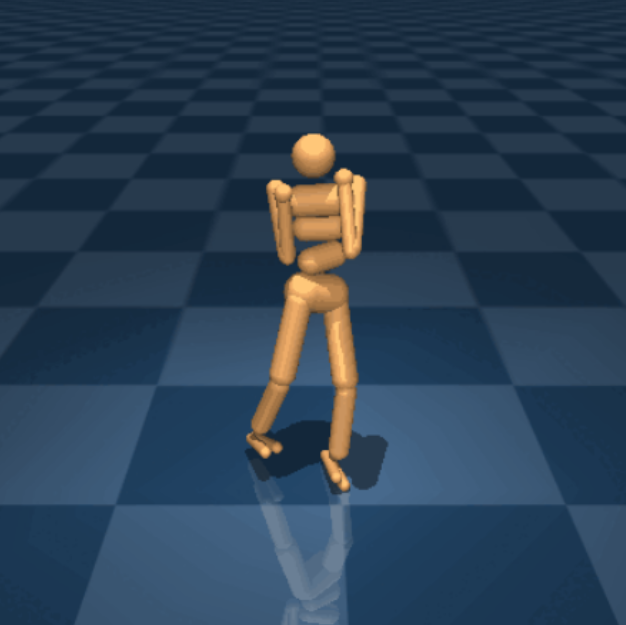
\includegraphics[height=10em]{figs/humanoid-1}};}] (i0) {};

  \node[mynode,minimum width=8em,minimum height=8em,outer sep=0,above of=e1,node distance=6em,path picture={\node at (path picture bounding box.center){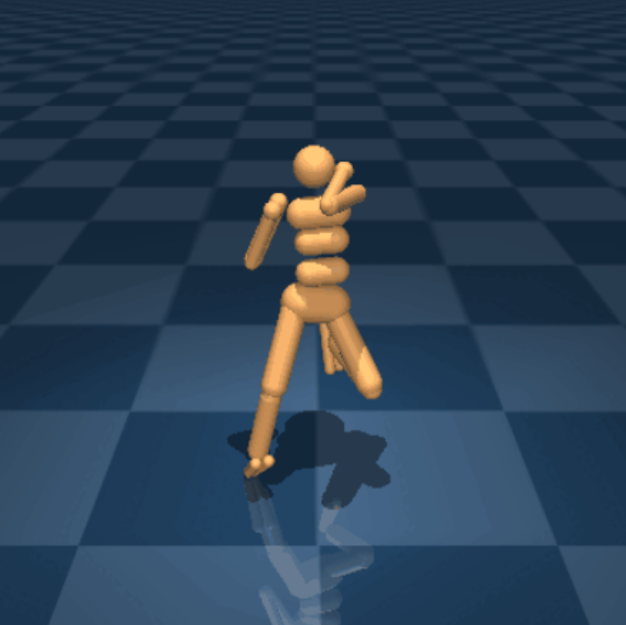
\includegraphics[height=10em]{figs/humanoid-3}};}] (i1) {};

  \node[mynode,minimum width=8em,minimum height=8em,outer sep=0,above of=e2,node distance=6em,path picture={\node at (path picture bounding box.center){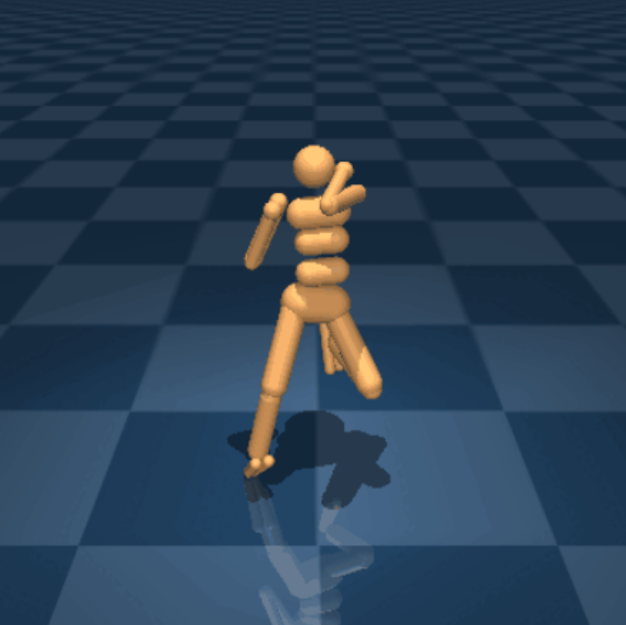
\includegraphics[height=10em]{figs/humanoid-3}};}] (i2) {};

  \node[anchor=north] (o0) at (i0.north) {\color{white}$o_{\sub}$};
  \node[anchor=north] (o1) at (i1.north) {\color{white}$o_{\subs{1}}$};
  \node[anchor=north] (o2) at (i2.north) {\color{white}$o_{\subs{2}}$};

  % Draw arrows
  \draw[arr] (i0) -- (e0);
  \draw[arr] (i1) -- (e1);
  \draw[arr] (i2) -- (e2);
  \draw[arr] (z0) -- node[below,font=\tiny] {Dynamics} (z1);
  \draw[arr] (z1) -- node[below,font=\tiny] {Dynamics} (z2);
  \draw[arr] (e0) -- node[above,font=\tiny,rotate=90,yshift=6pt] {Normalization} (z0);
  \draw[arr] (e1) -- (zh1);
  \draw[arr] (e2) -- (zh2);
  \draw[arr] (a0) -- (z1);
  \draw[arr] (a1) -- (z2);
  \draw[darr] (zh1) -- (z1);
  \draw[darr] (zh2) -- (z2);
  \draw[arr,-] (z2) -- ($(e2.east)!(z2)!(e2.east)$);

  % Add normalization
  \node[circle,fill=white,inner sep=0] at ($(e0)!.5!(z0)$) {\cube};
  \node[circle,fill=white,inner sep=0] at ($(e1)!.5!(zh1)$) {\cube};
  \node[circle,fill=white,inner sep=0] at ($(e2)!.5!(zh2)$) {\cube};

  % Minimization
  \node[blue!50,below of=z1,align=center,font=\scriptsize,xshift=4em] (min) {minimize: $\|\bar\vz-\hat\vz\|^{2}_{2}$};
  \draw[blue!50,line width=1pt,shorten <=1mm,shorten >=1mm,->] (min) to[bend right=30] ($(z1)!.5!(zh1)$);
  \draw[blue!50,line width=1pt,shorten <=1mm,shorten >=1mm,->] (min) to[bend left=30] ($(z2)!.5!(zh2)$);


\end{tikzpicture}
\vskip -0.1in
\caption{\textbf{Overview of \our's representation learning} \our learns a representation solely with the latent-state consistency loss, \ie a self-predictive loss (see \cref{eq:rep-loss}). We follow Finite Scalar Quantization \citep[FSQ,][]{mentzerFiniteScalarQuantization2023} and bound the domain of our latent representation, \ie we normalize it (denoted by \cube). Our normalization results in an implicit codebook (whose size we can control) and helps prevent representation collapse.}
  % Importantly, this prevents representation collapse without needing loss terms to minimize errors in reward and/or value predictions.
  % As such, our representations are task-agnostic.
  %We denote our normalization scheme by \cube.}
\label{fig:diagram-self-predictive}
\vskip -0.2in
\end{figure}

\section{Introduction}
\label{intro}

Reinforcement learning  \citep[RL, \eg][]{sutton2018reinforcement} has shown much promise in games, animation, and robotics.
However, applying RL in real-world environments is challenging. The problem is two-fold,
{\em (i)}~handling high dimensional/complex observation spaces is non-trivial, and {\em (ii)}~deep RL typically requires millions of data points which can be unpractical (or costly), \ie it is very sample inefficient.\looseness-1

% Given such a latent space,
% Whilst these latent states are often lower dimensional this is not always
Many approaches have been proposed to improve sample efficiency in deep RL.
As \citet{laskinCURLContrastiveUnsupervised2020} highlighted, these can generally be divided into two streams of research:
{\em (i)} auxiliary tasks on the agent's observations and {\em (ii)}~world models that predict the future
\citep{haRecurrentWorldModels2018,hafnerLearning2019,hansenTemporalDifferenceLearning2022}.
In this work, we are interested in the first class of methods, which use auxiliary tasks to improve sample efficiency.
In particular, we focus on representation learning methods that compress observations into latent states.
Nevertheless, our representation learning borrows ideas from world models as it uses multi-step predictions in a
latent-space dynamics model to learn temporally consistent representations \citep{zhaoSimplifiedTemporalConsistency2023}.\looseness-1
% In particular, methods for compressing observations into latent states.%, aka representation learning.

Learning representations for RL has been investigated for decades
\citep{abelOptimalBehaviorApproximate2016,mannorDynamicAbstractionReinforcement2004,liUnifiedTheoryState2006,andreStateAbstractionProgrammable2002,deardenAbstractionApproximateDecisiontheoretic1997,singhReinforcementLearningSoft1994,higginsDefinitionDisentangledRepresentations2018,vanhoofStableReinforcementLearning2016,watterEmbedControlLocally2015,ghoshRepresentationsStableOffPolicy2020}.
However, these approaches are usually limited to simple environments.
Some approaches used unsupervised learning \citep[\eg\ VAE,][with reconstruction loss]{kingmaAutoEncoding2014} to acquire representations
\citep{finnDeepSpatialAutoencoders2016,higginsDARLAImprovingZeroShot2017,langeAutonomousReinforcementLearning2012,watterEmbedControlLocally2015}.
More recently, self-supervised learning (SSL) approaches (which do not reconstruct observations)
attempt to learn good features without labels \cite{anandUnsupervisedStateRepresentation2019}.
% Alternative approaches leverage contrastive losses to learn representations \cite{laskinCURLContrastiveUnsupervised2020}.



Recently, TD-MPC \citep{hansenTemporalDifferenceLearning2022} and TCRL \citep{zhaoSimplifiedTemporalConsistency2023}
have obtained state-of-the-art performance on continuous control benchmarks by learning
representations with self-supervised losses.
In particular, they leverage the latent-state consistency loss.
This requires an encoder $e_{\theta}$ which maps observations $o_{t}$ to latent states $z_{t}$ and a dynamics model $d_{\phi}$ which predicts
the next latent states $z_{t+1}$ given a latent state $z_{t}$ and an action $a_{t}$.
It then minimizes the distance between the next state predicted by the dynamics model $d_{\phi}(e_{\phi}(z_{t}), a_{t})$
and the next state predicted by the target encoder $e_{\bar{\phi}}(z_{t+1})$.
Self-supervised losses are susceptible to a problem known as representation collapse, where the encoder learns a constant
representation \cite{jingUnderstandingDimensionalCollapse2021}.
As such, it is common to combine the latent-state consistency loss with other loss terms, such as
minimizing the reward prediction error in the latent space
\citep{zhangLearningInvariantRepresentations2020,zhaoSimplifiedTemporalConsistency2023,hansenTemporalDifferenceLearning2022,geladaDeepMDPLearningContinuous2019,rezaei-shoshtariContinuousMDPHomomorphisms2022}.
This helps to prevent representation collapse at the cost of learning a task-specific representation.\looseness-1
% Typically it is combined with other loss terms such as reward or value prediction.

% To the best of our knowledge, all prior works that learn representations with objectives that depend on
% predicting the reward and/or value in the latent space
% \citep{zhangLearningInvariantRepresentations2020,zhaoSimplifiedTemporalConsistency2023,hansenTemporalDifferenceLearning2022,geladaDeepMDPLearningContinuous2019,rezaei-shoshtariContinuousMDPHomomorphisms2022}.
% This is usually motivated by preventing representation collapse.
% To the best of our knowledge, all prior works that learn representations with objectives that depend on
% predicting the reward and/or value in the latent space
% \citep{zhangLearningInvariantRepresentations2020,zhaoSimplifiedTemporalConsistency2023,hansenTemporalDifferenceLearning2022,geladaDeepMDPLearningContinuous2019,rezaei-shoshtariContinuousMDPHomomorphisms2022}.
% This is usually motivated by preventing representation collapse.
% use a latent-state consistency loss based upon the Cosine
% For example, \citet{zhaoSimplifiedTemporalConsistency2023} use a latent-state consistency loss based upon the Cosine
% similarity loss plus the MSE of reward predictions in the latent space.
% The cosine similarity loss provides training stability whilst the reward prediction prevents representation collapse.
% However, learning representations using reward and/or value loss terms leads to the representations being task specific.

\begin{algorithm}[tb]
   \caption{\our}
   \label{alg:main_alg}
   \renewcommand{\algorithmiccomment}[1]{\hfill\textcolor{gray}{\(\triangleright\) #1}}
\begin{algorithmic}
   \STATE {\bfseries Input:} Encoder $e_{\theta}$, dynamics $d_{\phi}$, critics $\{Q_{\psi_{1}}, Q_{\psi_{2}} \}$, policy $\pi_{\eta}$, learning rate $\alpha$, target network update rate $\tau$
   \FOR{$i$ {\bfseries to} $N_{\text{episodes}}$}
    \STATE Collect data in environment:
    \STATE $\qquad \mathcal{D} \leftarrow \mathcal{D} \cup \{o_{t}, a_{t}, o_{t+1}, r_{t+1}\}^{T}_{t=0}$
    \FOR{$i=1$ {\bfseries to} $T$}
        \STATE Update representation:
        \STATE $\qquad [\theta, \phi] \leftarrow [\theta, \phi] + \alpha \nabla \left( \mathcal{L}_{\text{rep}}(\theta, \phi; \mathcal{D}) \right)$  \COMMENT{\cref{eq:rep-loss}}
        \STATE Update critic
        \STATE \quad \quad $\psi \leftarrow \psi + \alpha \nabla \left( \mathcal{L}_{Q}(\psi; \mathcal{D}) \right)$ \COMMENT{\cref{eq:value-loss}}
        \IF{$i$ \% 2 == 0}
          \STATE Update actor less frequently than critic:
          \STATE $\quad \quad \eta \leftarrow \psi + \alpha \nabla \left( \mathcal{L}_{\pi}(\psi; \mathcal{D}) \right)$  \COMMENT{\cref{eq:policy-loss}}
          % \STATE $\bar{\eta} \leftarrow \tau \bar{\eta} + (1-\tau) \eta$
        \ENDIF
        \STATE Update target networks:
        \STATE $\quad \quad [\bar{\theta}, \bar{\phi}, \bar{\psi}] \leftarrow \tau [\bar{\theta}, \bar{\phi}, \bar{\psi}] + (1-\tau) [{\theta}, {\phi}, {\psi}]$
    \ENDFOR
   \ENDFOR
\end{algorithmic}
\end{algorithm}


In this paper, we propose a simple representation learning technique that can be combined with any model-free RL method
\citep[we use TD3][]{fujimotoAddressingFunctionApproximation2018}.
See \cref{fig:diagram-self-predictive} for an overview of our (extremely simple) representation learning method.
It is based solely on the latent-state consistency loss, \ie a commonly used self-supervised loss for continuous RL.
In contrast to prior works, we normalize our latent representation using the technique from Finite Scalar Quantization
\citep{mentzerFiniteScalarQuantization2023}.
As a result, our latent space is bounded and associated with an \emph{implicit} codebook, whose size we can control.
% As a result, our latent space is associated with an \textit{implicit} codebook, whose size we can control.
Importantly, our method {\em (i)}~alleviates representation collapse,
{\em (ii)}~demonstrates state-of-the-art sample efficiency in continuous control benchmarks,
{\em (iii)}~is simple to implement, and {\em (iv)}~learns a task-agnostic
representation that could be helpful in downstream tasks.

\section{Related Work}
\label{sec:related_work}
In this section, we provide an overview of sample efficiency in RL.
Importantly, we recap how representation learning enabled model-free RL methods to obtain
state-of-the-art sample efficiency.

\textbf{Model-based RL}
Model-based RL (MBRL) is often said to be more sample efficient than model-free methods.
% This is because it can reason about the world and maximize the fraction of the information stream utilized for learning by utilizing the observations
This is because it learns a model in which it can reason about the world,
instead of simply trying to learn a policy or a value function to maximize the return \cite{haRecurrentWorldModels2018}.
% The world model can be used for planning \cite{allen1983planning, basye1992decision}.
A prominent idea has been to optimize the evidence lower bound of observation and reward sequences to learn world models that operate on the latent space of a learned Variational Autoencoder  \citep[VAE,][]{kingmaAutoEncoding2014, igl2018deep}. These models rely on maximizing the conditional observation likelihood $p(o_t | s_t$), which is the reconstruction objective.
The latent space of the model can be used for both planning with model-predictive control \cite{rubinstein1997optimization, hafnerLearning2019} or policy learning in the imagination of the world model \cite{hafner2019dream}. \citet{finn2017deep} and \citet{ebert2018visual} show that it is possible to plan with models that have been taught to predict videos directly without a VAE-based latent space.
% Incorporating the model uncertainty into planning through ensembling or sampling can also have a significant positive impact on the performance of model-based RL agents \cite{deisenrothPILCO2011, chua2018deep, janner2019trust, yu2020mopo, clavera2020model}.

Maximizing the ELBO or video reconstruction error to learn a world model can mislead the model to focus on learning task-irrelevant information, which distorts the optimization landscape \cite{zhang2018natural,zintgraf2021varibad}. When the task is complex, planning with reconstruction-based world models is unreliable \cite{lutter2021learning} and struggles to outperform model-free methods \cite{kostrikov2020image, yarats2021mastering}. The problems are aggravated when the environment is partially observable \cite{morad2023popgym}. Planning can be done through models that learn to predict rewards and values for multi-step rollouts \cite {tamar2016value, silver2017predictron, oh2017value, schrittwieser2020mastering}. However, these methods do not utilize the observations for model learning, making them inefficient.



\begin{figure*}[ht]
\vskip 0.2in
\begin{center}
\centerline{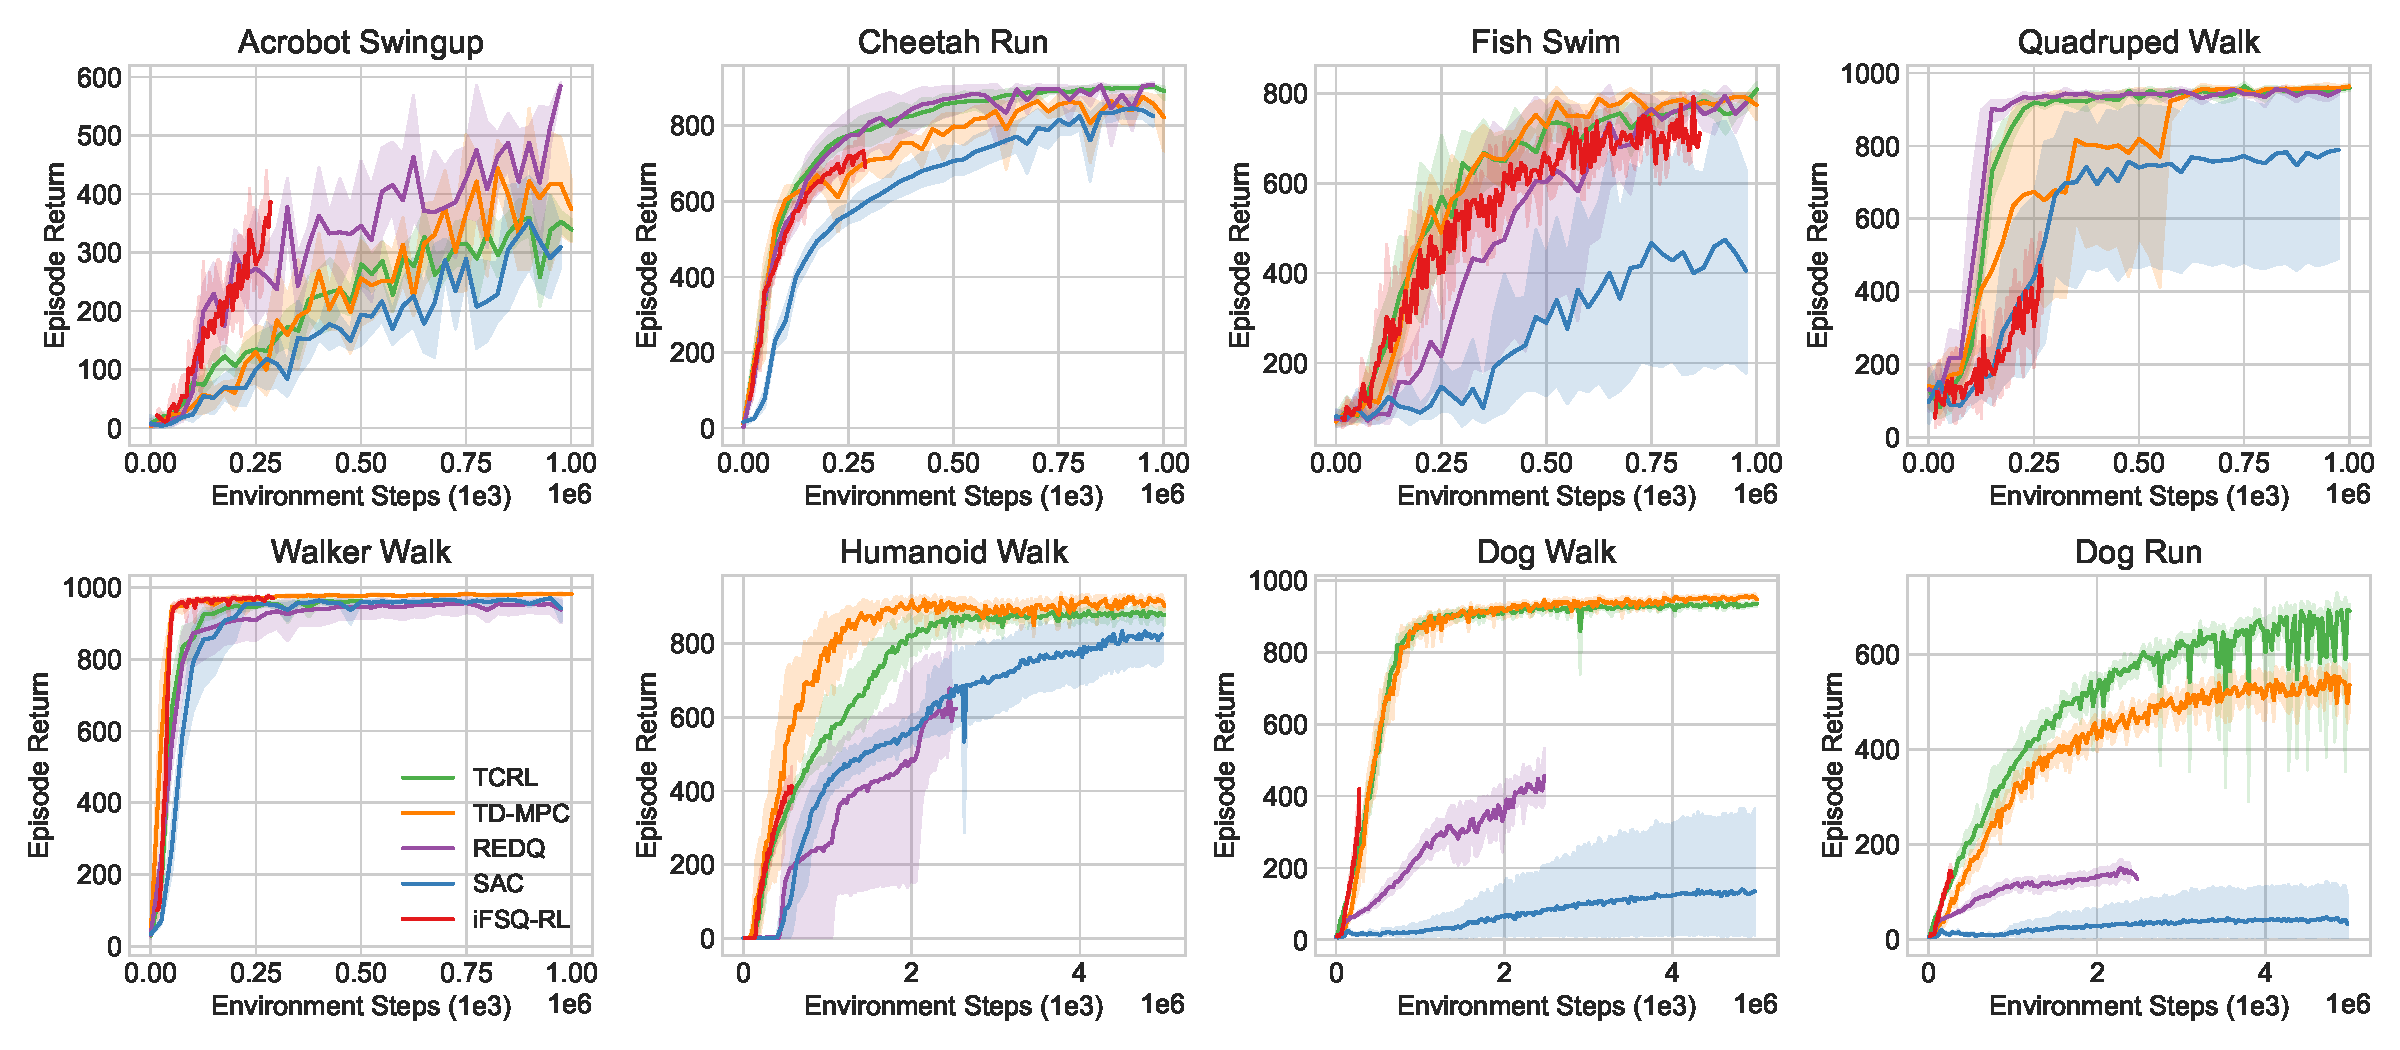
\includegraphics[width=1.0\textwidth]{./figs/baselines_comparison.pdf}}
\caption{\textbf{\our is simple, fast, and performant} \our is significantly more sample efficient than the model-free baselines SAC (blue) and REDQ (purple). It performs similarly to TD-MPC (orange) whilst being significantly simpler and quicker to train. \our even outperforms TCRL, which is the most similar baseline. Results are for seven DMC tasks with UTD=1. We plot the mean (solid line) and the $95\%$ confidence intervals (shaded) across 5 random seeds, where each seed averages over 10 evaluation episodes.}

\label{fig:normalization_improves_sample_efficiency}
\end{center}
\vskip -0.2in
\end{figure*}


\textbf{Self-predictive abstractions}
How can high-dimensional and noisy observations be used efficiently in model-based RL without resorting to reconstruction or direct prediction of future frames? A common solution has been to attach an auxiliary loss to the RL objective and perform representation learning \cite{tomar2021learning, ni2024bridging}. A promising approach for learning suitable representations is the use of self-predictive abstractions, where the model is trained to predict future latent states through an auxiliary loss \cite{subramanian2022approximate}. \citet{ye2021mastering} introduce a self-supervised consistency loss on the learned latent representations. Instead of relying on a reconstruction-based loss function, \citet{schwarzer2020data} propose a cosine similarity loss between predicted future latents and the true future latents and then perform Q-learning in the
learned latent space.\looseness-2
% \citet{ma2021contrastive} modify the classical world model learning objective by replacing the observation reconstruction loss with a contrastive learning term, which maximizes the mutual information between latent states and observations, helping combat the model focusing on learning task-irrelevant information. \citet{kipf2019contrastive} use contrastive learning to learn a structured world model. \citet{ghugare2022simplifying} argue that aligning the auxiliary objectives and RL objective can be difficult. The authors derive a bound directly on the overall RL objective, which is compatible with self-consistency. The contrastive objectives for model-based RL significantly improve sample efficiency, but they are not only limited to model-based RL. \citet{laskinCURLContrastiveUnsupervised2020} propose replacing the transition function with data augmentations to get a contrastive target and performing model-free learning using the representation produced by the encoder trained with the contrastive target.

\textbf{Latent-state consistency for model-based RL}
TD-MPC \cite{hansenTemporalDifferenceLearning2022} use a consistency loss to learn representations for planning with Model Predictive Path Integral control together with reward and value functions learned through temporal difference methods \cite{williams2015model}. TD-MPC2 \cite{hansen2023td} presents a series of improvements to TD-MPC to make the world model show scaling benefits and achieve state-of-the-art performance in a multi-task setting. They train world models with up to 317 million parameters and show monotone improvement in the normalized score across multiple environments and model sizes. The TD-MPC family of methods is applicable to real-world robotics \cite{lancaster2023modem} and learn representations that are suitable for transfer learning after adaptation \cite{yang2023movie} or fine-tuning \cite{feng2023finetuning}. \citet{zhu2023repo} demonstrate that the observation encoder can be made more resilient to spurious correlations by restricting the information flow from the observations to the latent representation, and the encoder can be easily aligned at test time in a reward-free manner.
% The loss function of TD-MPC can also be used to learn a manager in a hierarchical RL setting \cite{chitnis2023iql}.

\textbf{Latent-state consistency for model-free RL}
\citet{zhaoSimplifiedTemporalConsistency2023} show that the planning component of TD-MPC is not strictly necessary for high performance, and applying model-free learning on top of the self-consistent representations is sufficient for performance competitive with state-of-the-art. \citet{yuan2022euclid} propose using intrinsic rewards for pre-training temporally consistent models before using the rewards for adapting the world model for downstream tasks. We build on top of TCRL to show that we can combat the representation collapse through a normalization term and learn task-agnostic representations by dropping the reward term of the TCRL loss and only utilizing a multistep temporal consistency loss.


\section{Method}
\label{sec:method}

In this section, we detail our method, titled \textit{implicitly Quantized Reinforcement Learning} (\our).
\our is conceptually simple, it {\em (i)}~learns a representation of the observation space and then,
{\em (ii)}~performs model-free RL (\eg, TD3) on this representation.
% It the first representation learning phase, it learns an encoder which maps observations $o \in \mathcal{O}$
% to a latent space $z \in \mathcal{Z}$.
% It first learns a representation of the observation space and then uses
See \cref{fig:diagram-self-predictive} and \cref{alg:main_alg}.


\begin{figure*}[ht]
\vskip 0.2in
\begin{center}
\centerline{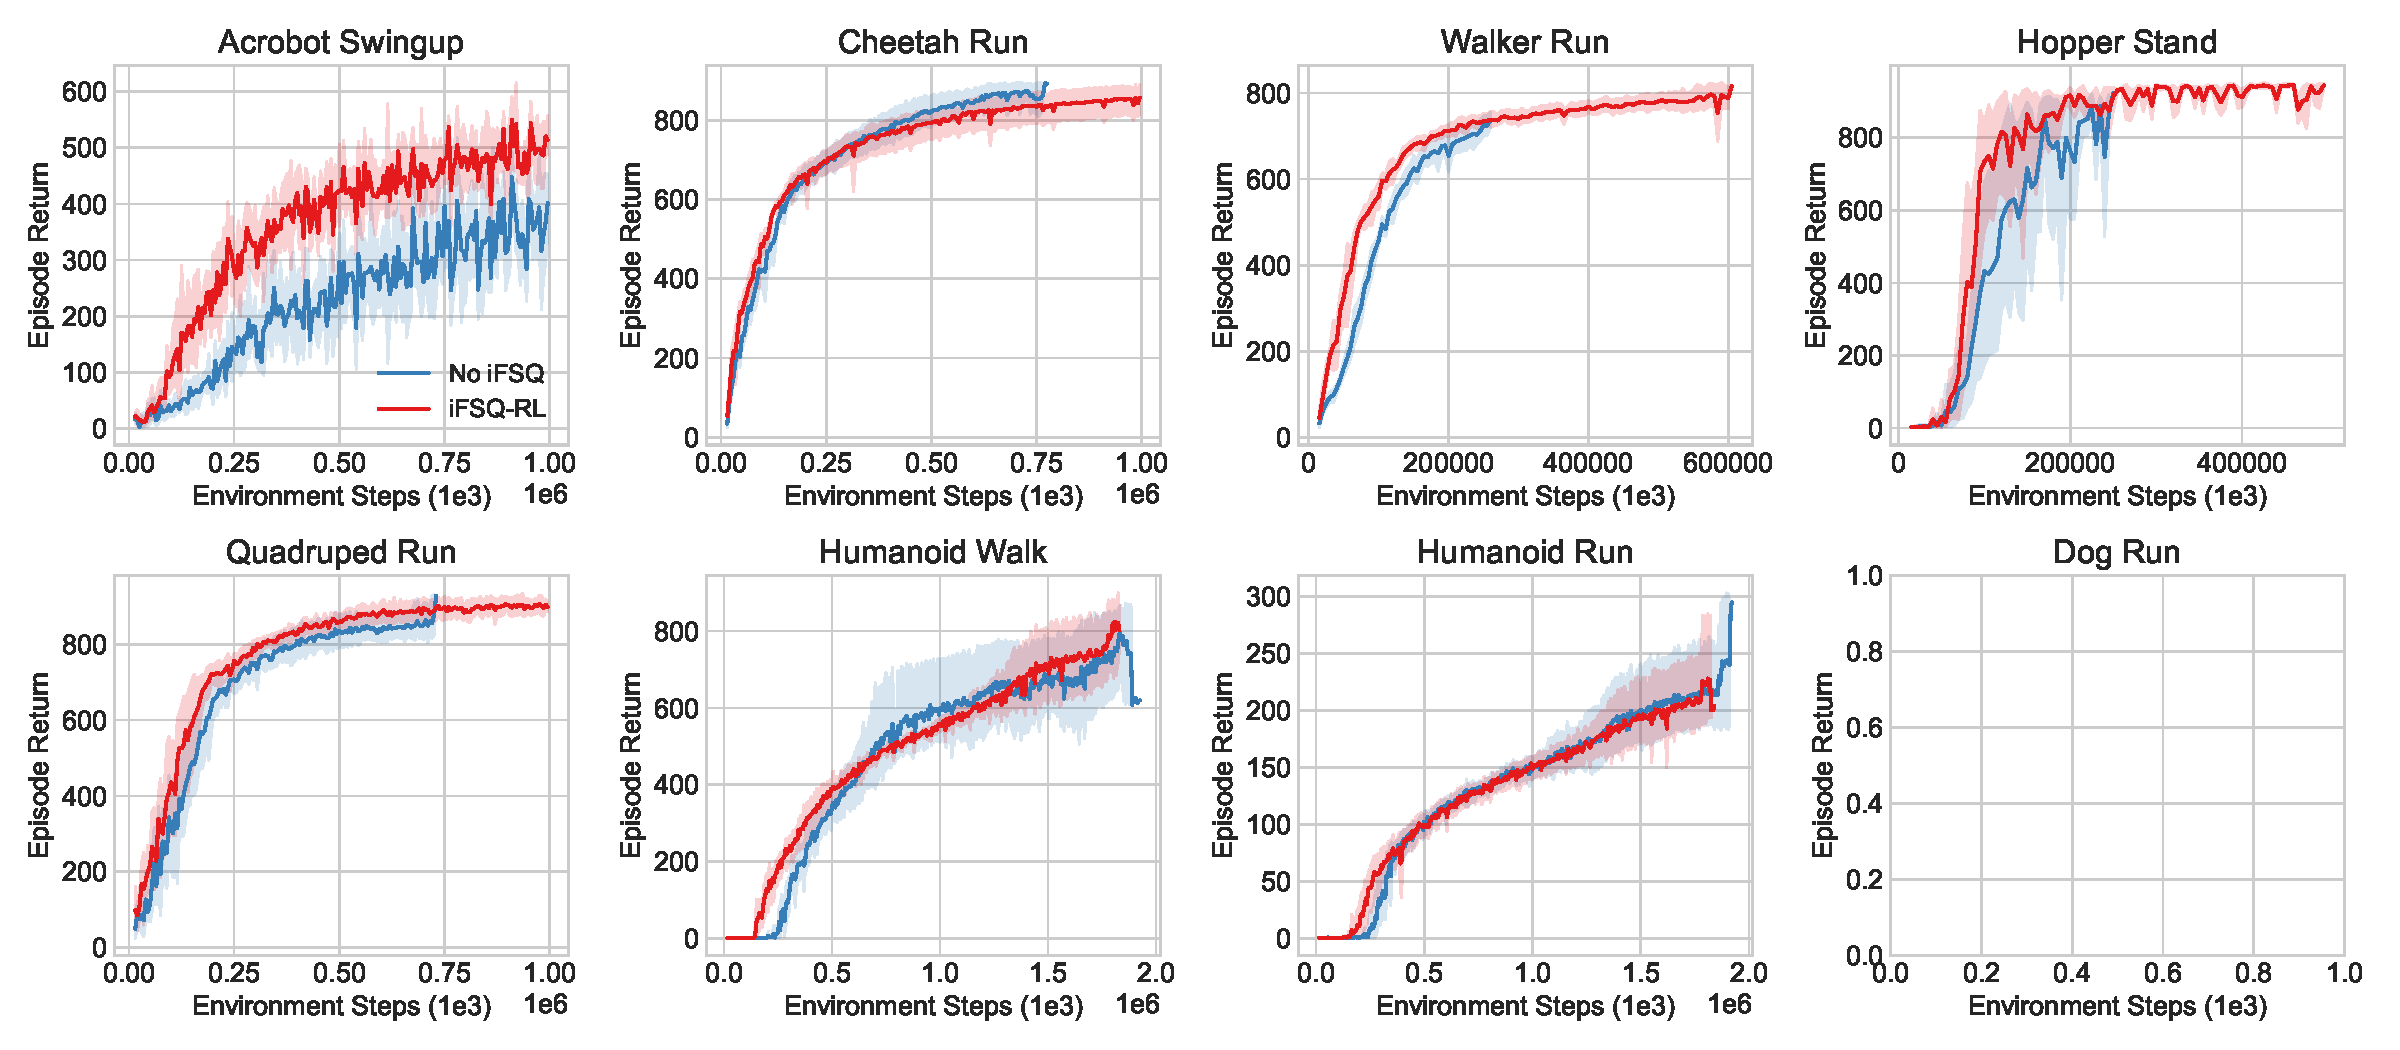
\includegraphics[width=1.0\textwidth]{./figs/normalization-ablation.pdf}}
\caption{\textbf{Ablation of normalization}. We analyze the impact of our FSQ-based normalization scheme on the sample-efficiency of \our. We plot the mean (solid line) and the $95\%$ confidence intervals (shaded) across 5 random seeds, where each seed averages over 10 evaluation episodes.}
\label{fig:normalization-ablation}
\end{center}
\vskip -0.2in
\end{figure*}


We consider Markov Decision Processes \citep[MDPs,][]{bellmanMarkovianDecisionProcess1957a} $\mathcal{M} = (\mathcal{O}, \mathcal{A}, \mathcal{P}, \mathcal{R}, \gamma)$,
where an agent receives an observation $o_{t} \in \mathcal{O}$ at time step $t$ and performs an action $a_{t} \in \mathcal{A}$.
The agent then obtains a reward $r_{t} = \mathcal{R} (o_{t}, a_{t})$ and obtains the next observation
$o_{t+1} = P(\cdot \mid o_{t}, a_{t})$.
The discount factor is denoted $\gamma \in [0, 1]$.





\textbf{Method overview}
\our has four main components which we wish to learn:
\begin{align}
&\text{Encoder: } & z_{t} &= e_{\theta} (s_{t}) \label{eq:encoder} \\
&\text{Dynamics: } & \hat{z}_{t+1} &= d_{\phi} (z_{t}, a_{t}) \label{eq:transition} \\
&\text{Value: } & q_{t} &= Q_{\psi} (z_{t}, a_{t}) \label{eq:value} \\
&\text{Policy: } & a_{t} &\sim \pi_{\eta} (z_{t}) . \label{eq:policy}
\end{align}
The encoder $e_{\theta}$  and latent-space dynamics model $d_{\phi}$ are responsible for representation learning.
The encoder $e_{\theta}$ maps observations $o_{t}$ to latent states $z_{t}$ and is responsible for learning a representation
which can aid RL.
The latent-space dynamics model $d_{\phi}$ predicts the next latent states $z_{t+1}$ given a latent state $z_{t}$ and an action $a_{t}$.
Its sole purpose is to aid representation learning by making the latent states temporally consistent.
Note that we do not use it for model-based RL.
Once we have the representation learned by our encoder, we map all observations to the latent space and perform model-free RL
in this latent space.
Throughout this paper, we use Twin Delayed Deep Deterministic Policy Gradient
(TD3), \citep{fujimotoAddressingFunctionApproximation2018}).
It consists of two state-action value functions $\{Q_{\psi_{1}},Q_{\psi_{2}} \}$, known as critics, and a deterministic
actor $\pi_{\eta}$.
Following prior works \citep{yaratsMasteringVisualContinuous2021}, we use a linear exploration noise schedule
which decays from $1$ to $0.1$ during training.



\textbf{Representation learning}
Our representation learning is based solely on the latent-state consistency loss,
%
\begin{align} \label{eq:rep-loss}
  \mathcal{L}_{\text{rep}}(\theta, \phi; \tau)
 % &= \E_{s_{t} \sim \mathcal{D}} \left[ \sum_{h=0}^{H-1} \| \hat{z}_{t+1} - z_{t+1} \|_{2}^{2} \right] \\
%&= \E_{(s_{t}, a_{t}, s_{t+1}) \sim \mathcal{D}}
% &= \E_{\tau \sim \mathcal{D}}
% \left[ \sum_{h=0}^{H-1} \gamma^{h} \| d_{\phi}(e_{\theta}(s_{t}), a_{t}) - e_{\bar{\theta}}(s_{t+1}) \|_{2}^{2} \right]
&= \sum_{h=0}^{H-1} \gamma^{h} \| d_{\phi}(\hat{z}_{t}, a_{t}) - e_{\bar{\theta}}(s_{t+1}) \|_{2}^{2},
\end{align}
%
which minimizes the distance between the next state predicted by the dynamics model $\hat{z}_{t+1} = d_{\phi}(\hat{z}_{t}, a_{t})$
and the next state predicted by the momentum encoder $\bar{z}_{t+1} = e_{\bar{\phi}}(s_{t+1})$.
The latent states are obtained with multi-step predictions in the latent space $\hat{z}_{t+1} = d(\hat{z}_{t}, a_{t})$
with $\hat{z}_{0} = e_{\theta}(s_{0})$.
The initial mapping to the latent space $\hat{z}_{0} = e_{\theta}(s_{0})$ uses the online encoder which
is being trained jointly with the dynamics model $d_{\phi}(\hat{z_{t}}, a_{t})$.
The target $e_{\bar{\phi}}(z_{t+1})$ is calculated with the momentum encoder which uses an exponential moving average (EMA)
of the encoder's weights $\bar{\theta} \leftarrow \tau \bar{\theta} + (1-\tau)\theta$.
% As such, gradient to not flow through the target network
The target network update rate is denoted $\tau$.

\begin{table}[t]
\caption{FSQ levels $\mathcal{L}$ to approximate different codebook sizes $|\mathcal{C}|$}
\label{tab:fsq-levels}
\vskip 0.15in
\begin{center}
\begin{small}
\begin{sc}
\begin{tabular}{lccc}
\toprule
Target size $|\mathcal{C}|$ & $2^{6}$ & $2^{8}$ & $2^{10}$ \\
\midrule
Proposed $\mathcal{L}$ & $[8,8]$ & $[8,6,5]$ & $[8,5,5,5]$ \\
% Target size $|\mathcal{C}|$ & $2^{8}$ & $2^{10}$ & $2^{12}$ \\
% \midrule
% Proposed $\mathcal{L}$ & $[8,6,5]$ & $[8,5,5,5]$ & $[7,5,5,5,5]$ \\
\bottomrule
\end{tabular}
\end{sc}
\end{small}
\end{center}
\vskip -0.1in
\end{table}

\begin{figure*}[ht]
\vskip 0.2in
\begin{center}
\centerline{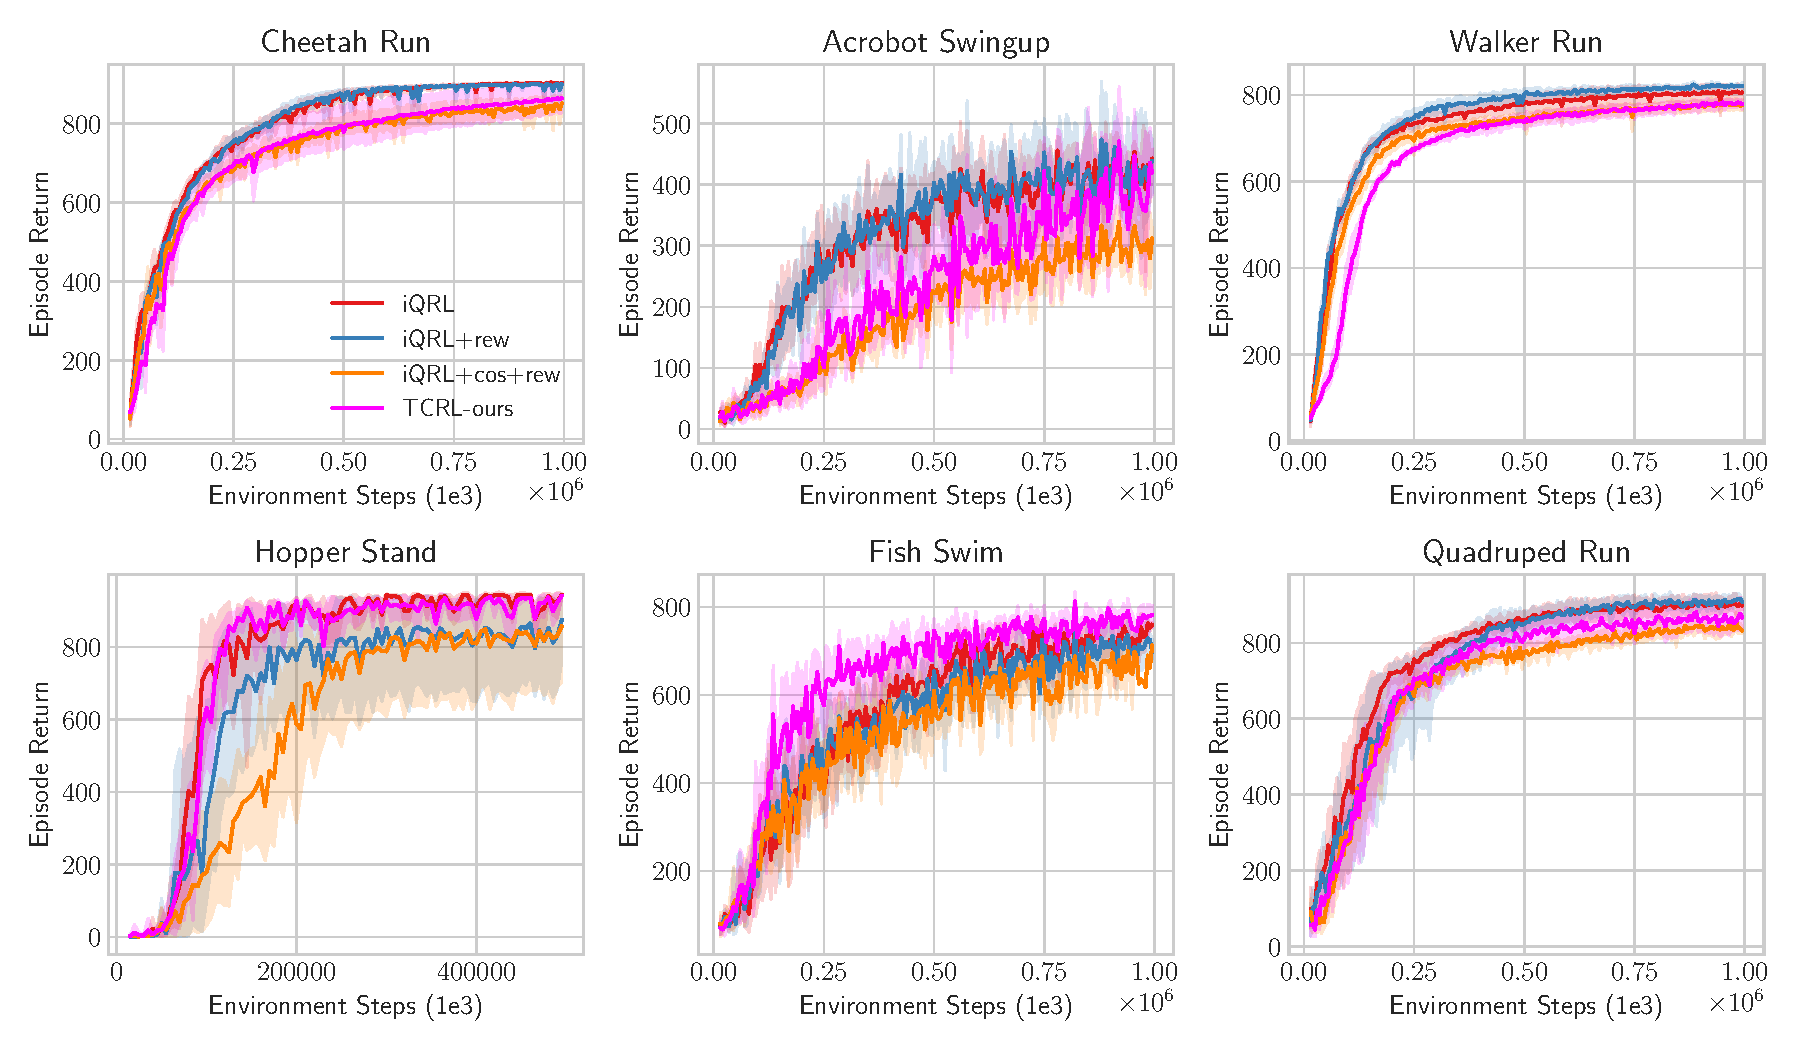
\includegraphics[width=0.9\textwidth]{./figs/reward-ablation.pdf}}
\caption{\textbf{Reward prediction is not necessary for representation learning}. We compare \our to variants of our method with a reward prediction term included in the representation learning loss. \our performs on par with the best method on all environments except Fish Swim, where it is slightly inferior to our version of TCRL. We plot the mean (solid line) and the $95\%$ confidence intervals (shaded) across 5 random seeds, where each seed averages over 10 evaluation episodes.}
\label{fig:reward-ablation}
\end{center}
\vskip -0.2in
\end{figure*}


\textbf{Normalization with implicit quantization}
% However, this can lead to exploding gradients and
Motivated by preventing representation collapse we seek a representation with high matrix rank.
To this end, we bound our latent space following the approach from
Finite Scalar Quantization \citep[FSQ,][]{mentzerFiniteScalarQuantization2023}.
Note that the latent state $z_{t}$ is typically a vector of unbounded real numbers, \ie $z_{t} \in \R^{d}$.
% each (scalar) entry in the representation $z_{t}$ is independently quantized to the nearest integer by rounding
Their important observation is that carefully bounding each channel gives rise to an implicit codebook of a chosen size.
Let's consider a single element of the latent state $z$ and give it $c$ channels so it's of shape $[c]$.
% Here $d$ is the output dimension of the NN.
Mapping each entry $z_{i}$ to $L$ values (\eg, via $z_{i} \rightarrow [L/2] \text{tanh}(z_{i})$ and rounding to integers),
obtains a quantized $\tilde{z} \in \mathcal{C}$, where $\tilde{z}$ takes one of $L^{c}$ unique possible vectors.
This gives rise to an implicit codebook $\mathcal{C}$ given by the product of the per-channel codebook sets.
% The size of the codebook $|\mathcal{C}| = L^{c}$ is given by the product of the
% For example, specifying $c=3$ channels
This idea generalizes to the case where the $i^{\text{th}}$ channel is mapped to $L_{i}$ values, giving a codebook of size $|\mathcal{C}| = L_{i}^{c_{i}}$.
% Since quantization is performed by rounding to integers

FSQ has the following hyperparameters: we must specify the number of channels $c$ and the number of levels per channel
$\mathcal{L} = [L_{1},\ldots,L_{c}]$.
\cref{tab:fsq-levels} shows the recommended number of channels and number of levels per channel to obtain codebooks of different sizes \citep{mentzerFiniteScalarQuantization2023}.
FSQ, relies on a simple, fixed grid partition in a much
lower-dimensional space.
In practice, we found codebooks of size $|\mathcal{C}|=2^{6}$ sufficient for most environments in the DeepMind Control suite.
However, for the Dog Walk environment we used a codebook of size $|\mathcal{C}|=2^{8}$.

% Fig. 1 shows FSQ for d=3, L=3, implying a codebook
% C = {(−1, −1, −1),(−1, −1, 0),(−1, −1, 1), . . . ,(1, 1, 1)}, where |C| = L
% d = 27.


% However, thi w
% bounding the range of the quantizer
% However, in our work we bound the domain of the latent space, \ie $z_{t} \in [-L, L]^{d}$.
% We follow Finite Scalar Quantization (FSQ, \cite{mentzerFiniteScalarQuantization2023})
% and bound each dimension of our latent space.
% Given the output of our MLP encoder $z \in \R^{d}$,

% where each entry in  $f : z \rightarrow \left[ L/2 \right] \mathrm{tanh}(z))$

% Unlike previous works, we normalize the latent vector

% \textbf{Bounding the latent space}


% Thereby, we have zˆ ∈ C, where C is the implied codebook, given by the product of these per-channel
% codebook sets, with |C| = L
% d
% . The vectors in C can simply be enumerated leading to a bijection from
% any zˆ to an integer in {1, . . . , Ld}. Therefore, VQ can be replaced with FSQ in any neural networkrelated setup where VQ is commonly used, e.g., to train transformers, after appropriately adapting
% the output and input dimension of the layers before and after VQ, respectively. We generalize the
% above exposition to the case where the i-th channel is mapped to Li values and get |C| =
% Qd
% i=1 Li


\begin{figure*}[ht]
	\vskip 0.2in
	\begin{center}
		\centerline{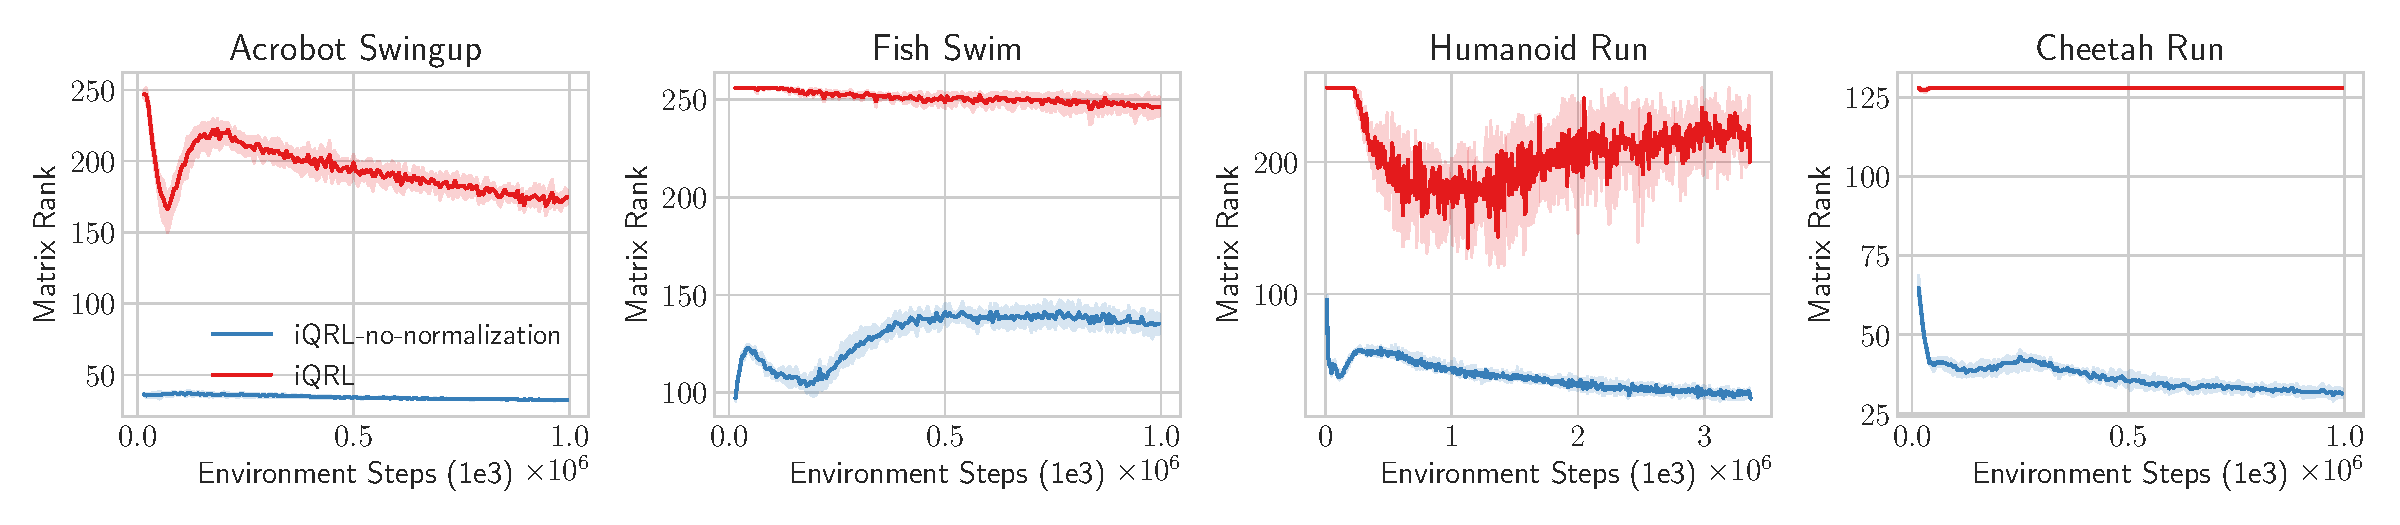
\includegraphics[width=1.0\textwidth]{./figs/rank-comparison-z1.pdf}}
		\caption{\textbf{Representation collapse without normalization}. We observe that the representation normalization of \our is crucial for avoiding representation collapse. When no normalization is applied to the latent variables, the matrix rank of the representations drops rapidly, which can hurt the downstream performance. We plot the mean (solid line) and the $95\%$ confidence intervals (shaded) across 5 random seeds, where each seed averages over 10 evaluation episodes.}
		\label{fig:rank-comparison-z1}
	\end{center}
	\vskip -0.2in
\end{figure*}



\textbf{Policy and value function learning}
We learn the policy and value function using TD3 \citep{fujimotoAddressingFunctionApproximation2018}.
However, we follow \citet{yaratsMasteringVisualContinuous2021,zhaoSimplifiedTemporalConsistency2023}
and augment the loss with n-step returns.
The only difference to TD3 is that instead of using the original observations $o_{t}$, we map them through the
target encoder $z_{t} = e_{\bar{\theta}}(o_{t})$ and learn the value function and policy in the latent space $z_{t}$.
The value function is updated by minimizing the following objective:
\begin{align} \label{eq:value-loss}
  \mathcal{L}_{Q} &= \E_{\tau \sim \mathcal{D}} \left[ (Q_{\psi_{k}}(e_{\bar{\theta}}(s_{t}), a_{t}) - y)^{2}  \right], \quad  \forall k \in 1, 2 \\
  y &= \sum_{n=0}^{N-1} \gamma^{n} r_{t+n} + \gamma^{n} \min_{k \in \{1,2\}} Q_{\bar{\psi}_{k}}(e_{\bar{\theta}}(s_{t+n}), a_{t+n}), \nonumber
\end{align}
where we use policy smoothing by adding clipped Gaussian noise $\epsilon_{t+n} \sim \mathcal{N} (0,\sigma^{2})$ to the
action $a_{t+n} = \pi_{\bar{\eta}}(z_{t+n}) + \epsilon_{t+n}$.
Note that we use the target encoder to get the latent states in both the prediction and the target.
We then use the target value functions $Q_{\bar{\psi}_{k}}$ and the target policy $\pi_{\bar{\eta}}$ to calculate the TD target.
Following TD3, we learn the actor's parameters by minimizing
%
\begin{align} \label{eq:policy-loss}
 \mathcal{L}_{\pi} = - \E_{(o_{t}, a_{t}) \sim \mathcal{D}} \left[ \min_{k\in\{1,2\}} Q_{\psi_{k}}(e_{\bar{\theta}}(o_{t}), a_{t}) \right].
\end{align}
%
That is, we maximize the Q-value using the clipped double Q learning trick to combat overestimation in Q learning.

% Whilst our method resembles TCRL \citep{zhaoSimplifiedTemporalConsistency2023} it is important to note that
% our transition model does not predict the reward.
% As such, our method learns a task-agnostic representation.





\section{Experiments}
\label{sec:experiments}
In this section, we evaluate \our in a variety of continuous control tasks from the DeepMind Control (DMC) Suite \cite{tassa2018deepmind}.
We aim to answer the following questions:
\begin{itemize}
    \item How does \our compare to state-of-the-art model-free and model-based algorithms?
    \item Does the FSQ-based normalization of \our help combat rank collapse of the learned latent-space representation?
    \item Is learning a representation with only latent-state consistency really better than including reward predictions and value predictions?
    \item Can \our's task-agnostic representation aid task adaptation with its pre-trained representation?
\end{itemize}

% \begin{figure*}[ht]
% \vskip 0.2in
% \begin{center}
% \centerline{\includegraphics[width=1.0\textwidth]{./figs/utd_comparison.pdf}}
% \caption{\textbf{Normalizing the latent-space enables higher UTD} \our's (blue) sample efficiency improves when the UTD ratio is increased from $1 \rightarrow 8$. TCRL (which has an un-normalized latent space) does not see an improvement in sample efficiency when when the UTD ratio is increased. Results are for four DMC tasks. We plot the mean (solid line) and the $95\%$ confidence intervals (shaded) across 5 random seeds, where each seed averages over 10 evaluation episodes.}
% \label{fig:normalization_enables_higher_utd}
% \end{center}
% \vskip -0.2in
% \end{figure*}

% \textbf{Normalizing the latent-space enables higher UTD}
% We first show how using bounded latent states enables us to increase the UTD ratio to see improvements in sample efficiency.
% \cref{fig:normalization_enables_higher_utd} shows that as the UTD ratio is increased from $1$ to $8$ \our's sample efficiency
% continues to improve.
% In contrast, when increasing the UTD ratio for TCRL no improvements are observed.

\textbf{\our is simple, fast, and performant}
In \cref{fig:normalization_improves_sample_efficiency}, we compare \our to the model-free baselines Soft-Actor Critic (SAC) \cite{haarnojaSoft2018} and Randomized Ensemble Double Q Learning (REDQ) \cite{chenRandomizedEnsembledDouble2021}, and the model-based baselines TD-MPC \cite{hansenTemporalDifferenceLearning2022} and TCRL \cite{zhaoSimplifiedTemporalConsistency2023} on seven problems from the DeepMind Control Suite. The results show that our method, \our, performs on par with TD-MPC while being significantly simpler and quicker to train, as the loss term consists of fewer terms and no planning is needed, unlike in TD-MPC. We even outperform TCRL, which is the most similar baseline to our work. We ablate the effect of the FSQ-based latent-space normalization scheme in \cref{fig:normalization-ablation}. The normalization is overall beneficial.

\textbf{\our does not suffer from rank collapse} We analyze the impact of the latent-space normalization on the rank of the latent representations outputted by the learned encoder.
We follow the methodology of \citet{ni2024bridging} for estimating the matrix rank. We plot the ranks in \cref{fig:rank-comparison-z1}. The latent state dimensions are 256, 256, 256, and 128 for Acrobot Swingup, Fish Swim, Humanoid Run, and Cheetah Run, respectively, and the plots show that the matrix rank stays close to the latent state dimension when our FSQ normalization scheme is applied. Without normalization, a dimensional collapse occurs, which can have significant harmful effects as the representational power of the latent state diminishes \cite{jingUnderstandingDimensionalCollapse2021}. Note that in contrast to \citet{ni2024bridging}, we observe that using a detached momentum encoder as the target encoder is insufficient to prevent a rank collapse in practice. We hypothesize that this is due to trivial representations being enough to minimize the prediction error when a reward term is not present in the loss \cite{tang2023understanding}. 

\begin{figure*}[ht]
	\vskip 0.2in
	\begin{center}
		\centerline{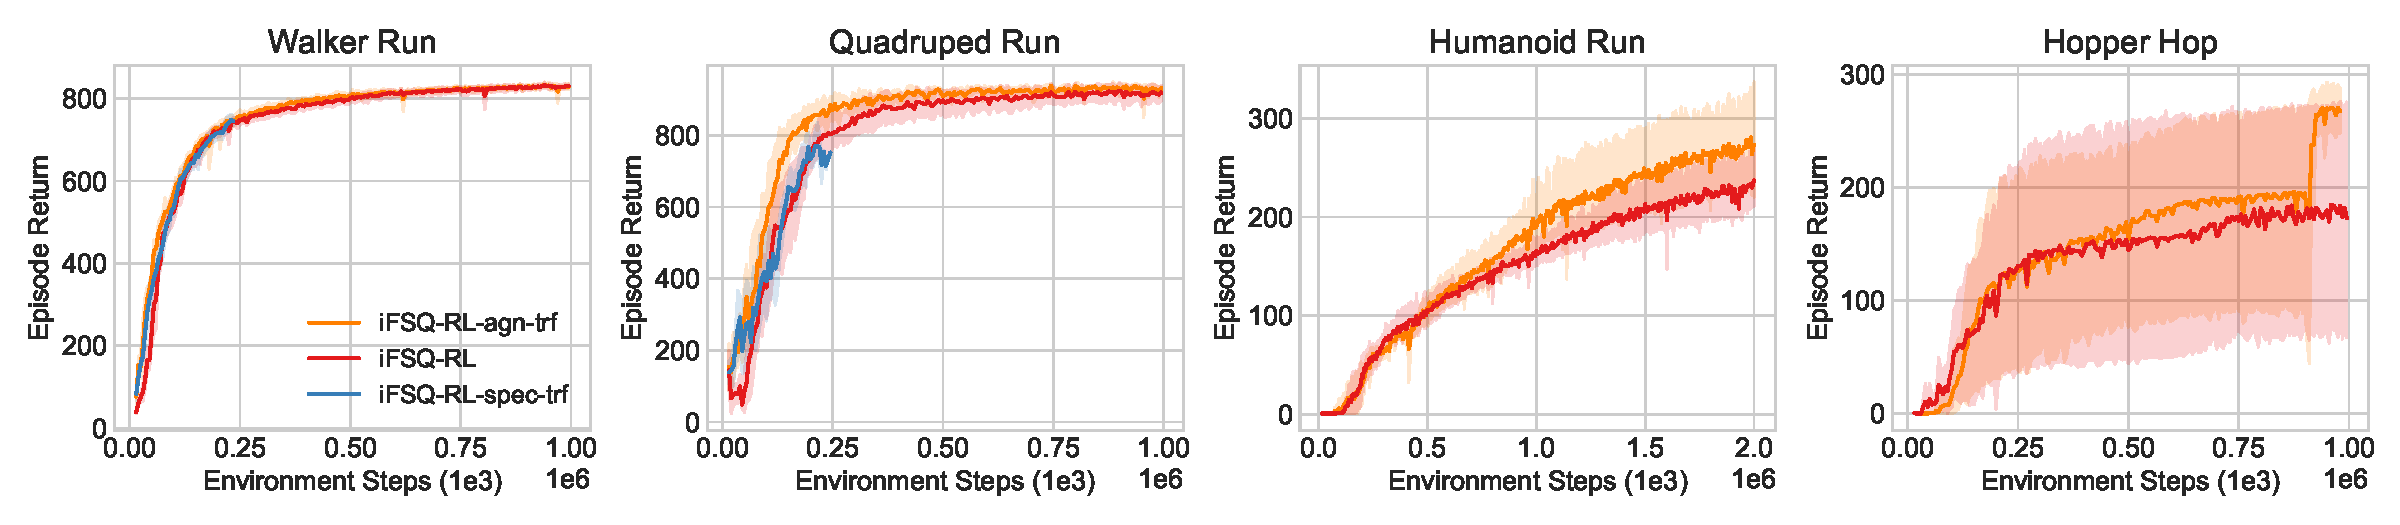
\includegraphics[width=0.8\textwidth]{./figs/task-agnostic-ablation.pdf}}
		\caption{\textbf{\our's task-agnostic representation helps for multi-task RL}. We evaluate whether pre-training \our on the walk tasks in the DeepMind Control Suite help for learning the run task on the same environment. The pre-training proves to be beneficial on all evaluated environments. If the representation is task-specific, \ie the reward prediction term is included, the pre-training can be clearly detrimental. We plot the mean (solid line) and the $95\%$ confidence intervals (shaded) across 5 random seeds, where each seed averages over 10 evaluation episodes.}
		\label{fig:multi-task-pretraining}
	\end{center}
	\vskip -0.2in
\end{figure*}


\begin{figure*}[ht]
	\vskip 0.2in
	\begin{center}
		\centerline{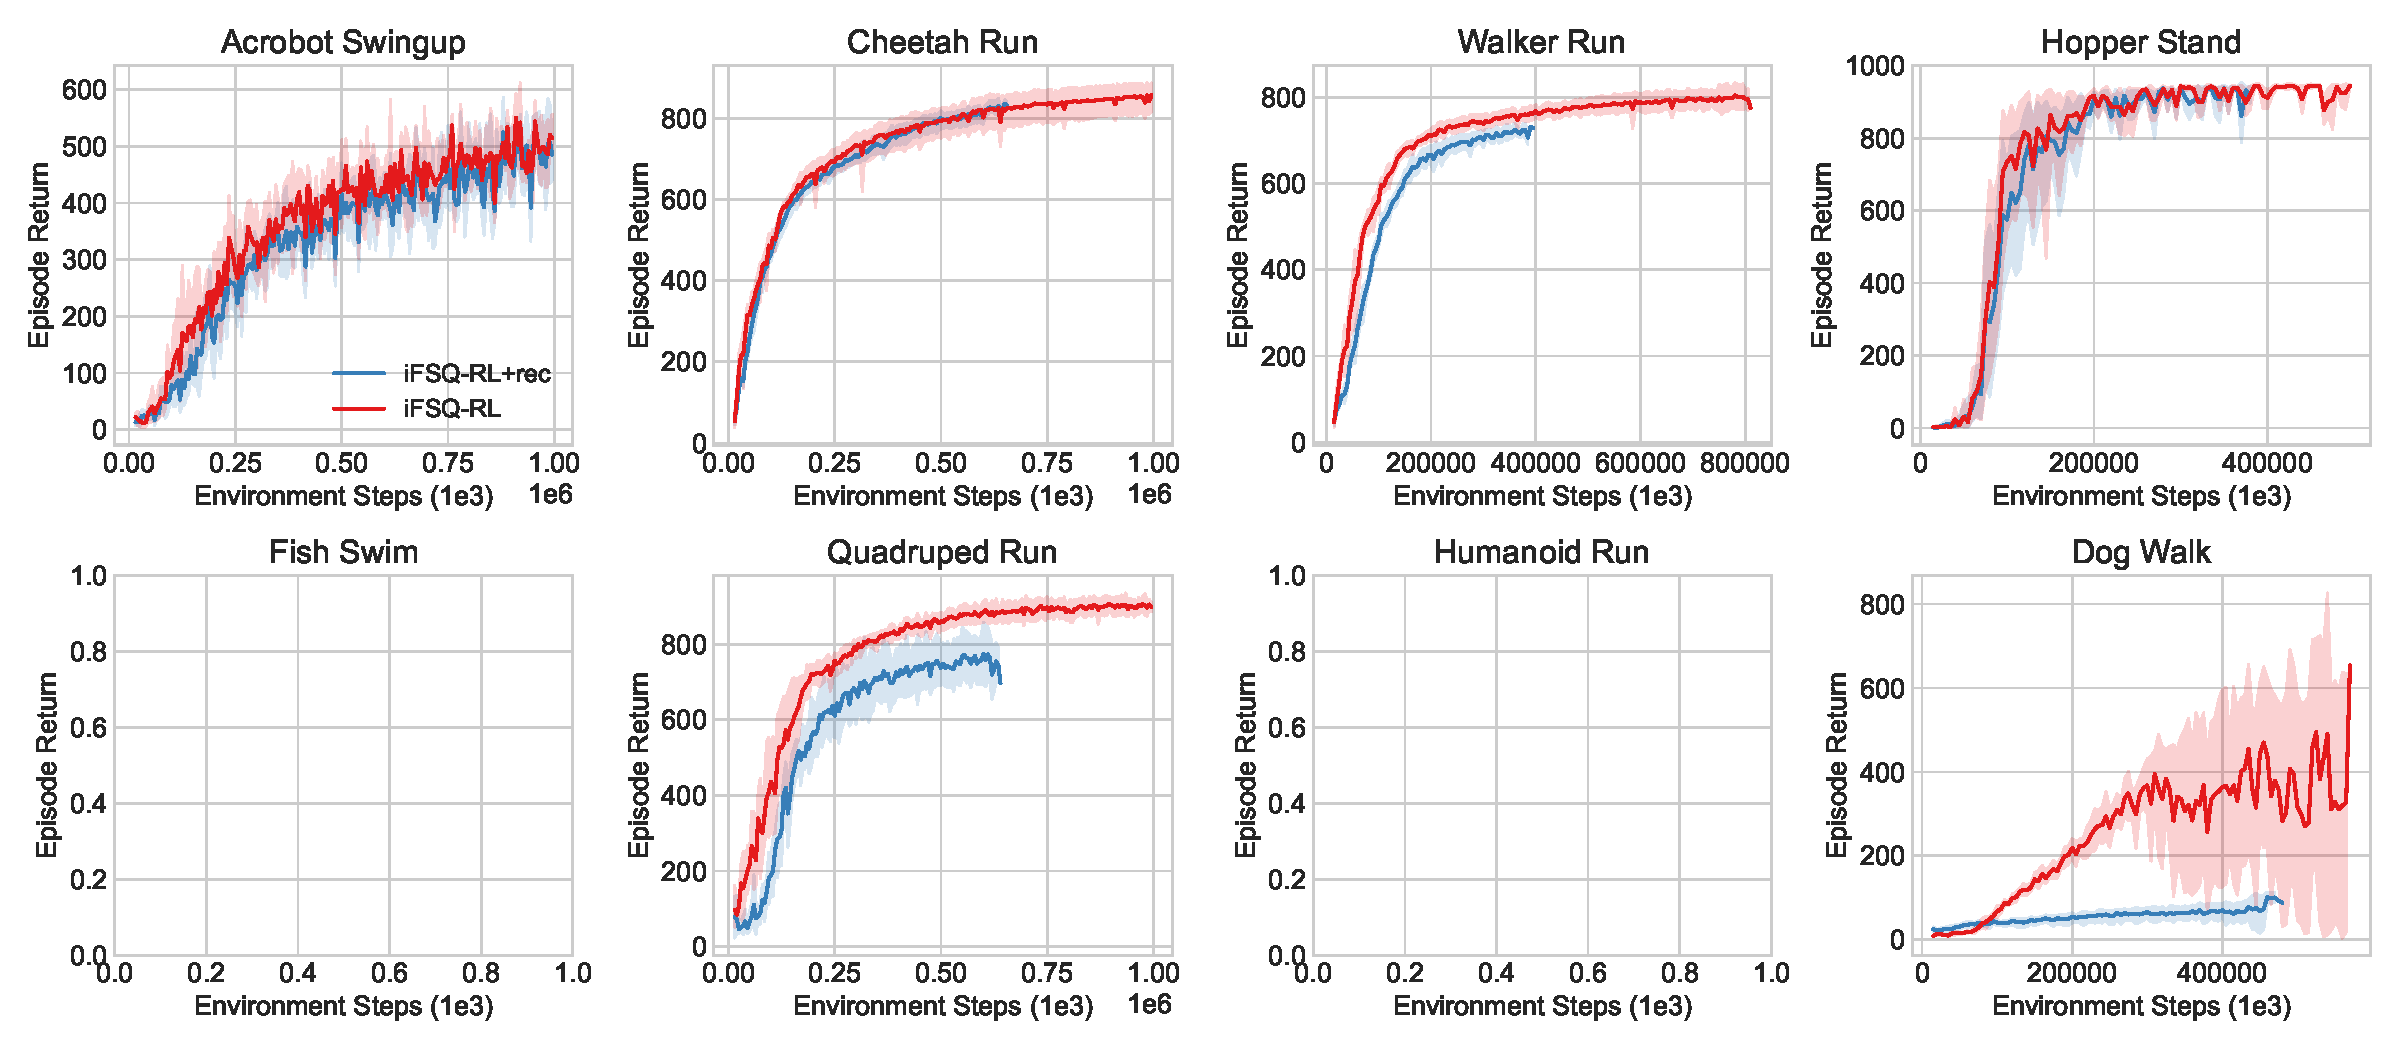
\includegraphics[width=1.0\textwidth]{./figs/reconstruction-loss-ablation.pdf}}
		\caption{\textbf{Reconstruction loss has detrimental impact}. Unlike many methods, such as Dreamer-v3 \cite{hafner2023mastering}, \our neither has an observation decoder nor a reconstruction term in the loss function. We show that adding a reconstruction loss harms the performance of \our across all evaluation environments. We plot the mean (solid line) and the $95\%$ confidence intervals (shaded) across 5 random seeds, where each seed averages over 10 evaluation episodes.}
		\label{fig:reconstruction-loss-ablation}
	\end{center}
	\vskip -0.2in
\end{figure*}

\textbf{Reward prediction is not necessary for representation learning}
Unlike prior methods such as TCLR \cite{zhaoSimplifiedTemporalConsistency2023}, TD-MPC \cite{hansenTemporalDifferenceLearning2022}, and Dreamer-V2 \cite{hafnerMasteringAtariDiscrete2022}, our representation learningloss (\cref{eq:rep-loss}) does not include a term for learning to predict the reward or the value. Instead, we rely solely on the self-predictive temporal consistency loss. To analyze the impact of not including the reward prediction term, we perform an ablation study, where we compare our method to three variants of our method:
\begin{itemize}
	\item \ourrew, where we add a reward prediction head into our model architecture by re-defining the dynamics as $\hat{z}_{t+1}, \hat{r}_t = d_{\phi} (z_{t}, a_{t})$ (see \cref{eq:transition}), and include a reward prediction term (discounted MSE Loss) in the representation loss:
	\begin{align*}
		\mathcal{L}_\text{rew} = \sum_{h=0}^{H-1} \gamma^h \| \hat{r}_{t+h} - r_{t+h}\|_2^2,
	\end{align*}
	where $r_{t+h}$ is the ground-truth H-step reward and $\hat{r}_{t+h}$ the predicted H-step rewards.
	\item \ourcosrew, where in addition to the reward prediction head in \ourrew, we additionally convert the self-supervised MSE loss (see \cref{eq:rep-loss}) for the temporal consistency into a cosine similarity, similarly to TCRL:
	\begin{align*} \label{eq:rep-loss}
		\mathcal{L}_{\text{rep}}(\theta, \phi; \tau)
		&= - \sum_{h=0}^{H-1} \gamma^{h} \left ( \frac{\hat{z}_{t+h}}{\| \hat{z}_{t+h} \|_2} \right )^T \left ( \frac{\tilde{z}_{t+h}}{\| \tilde{z}_{t+h} \|_2} \right ),
	\end{align*}
  where as before we have $\hat{z}_{t+h} = d_{\phi}(\hat{z}_{t}, a_{t})$ and $\tilde{z}_{t+h} = e_{\bar{\theta}}(s_{t+1})$.
	\item TCRL-ours, where in addition to \ourcosrew, we remove the FSQ normalization scheme to make the method equal to TCRL with some minor improvements to the method, such as using nstep-TD3 \cite{fujimotoAddressingFunctionApproximation2018} as the base algorithm instead of DDPG with Double Q and nstep returns, using the neural network architecture from \citet{hansen2023td}, and performing policy smoothing \cite{fujimotoAddressingFunctionApproximation2018}.
\end{itemize}
The results for this ablation study are shown in \cref{fig:reward-ablation}. 
The plots show that our method, \our, without a reward prediction term in the loss, has equal or superior performance to the comparison methods except in Fish Swim, where the unnormalized TCRL-ours outperforms all the methods with normalization due to being able to maintain the latent matrix rank in this specific environment (see \cref{fig:rank-comparison-z1}). Even then, \our performs equally to the normalized variants of our method with the reward prediction. Our results imply that learning to predict the reward is not necessary for learning a suitable latent representation. The upside of not including the reward prediction head is that it makes the representation task-agnostic, which we believe to be important for downstream applications such as learning in an incremental multi-task setting.

\textbf{\our's task-agnostic representation is helpful for multi-task RL}
In contrast to \eg TCRL \cite{zhaoSimplifiedTemporalConsistency2023} and TD-MPC \cite{hansenTemporalDifferenceLearning2022}, \our learns a representation that is task-agnostic, that is, there are no task-specific components such as reward or value prediction in the representation loss (\cref{eq:rep-loss}). The potential upside of \our's task-agnostic representation is it can be used to speed up learning in the incremental multi-task setting. That is, we can leverage the representation learned from solving one task to aid in learning other tasks in the same domain. For instance, we can pre-train a representation in Walker Walk and use it to speed up the training process in Walker Run. The only requirement is that the action and observation spaces must match. In addition, we assume that the transition dynamics are unchanged, but the reward may change.

We evaluate whether pre-trained representations are beneficial in three environments. We start by pre-training \our on Walker Walk, Quadruped Walk, and Humanoid Walk. In addition, we replicate the pre-training on Walker Walk and Quadruped Walk by adding a reward prediction term to the representation loss. Then, we retain the encoder and dynamics function from the pre-training and train \our on the target tasks Walker Run, Quadruped Run, and Humanoid Run. We compare the pre-trained agents to training \our on these tasks from scratch. The results for this experiment are shown in \cref{fig:multi-task-pretraining}.

The plots in \cref{fig:multi-task-pretraining} show that when the encoder and the dynamics function have been pre-trained, the agent learns quicker than when it is trained from scratch. This effect is particularly visible in Quadruped Run and Humanoid Run. In contrast, when the reward term has been included in the pre-training objective, making the representation task-specific, the pre-training proves to be harmful on Quadruped Run. This indicates that \our's task-agnostic representation is beneficial in continual and lifelong learning settings.
% However, given the breadth of

% we show that \our can benefit from pre-training the representation in a different environment with the same dynamics. In contrast, if the representation learning objective used 

%pre-training objective contains 

%That is, leveraging information learned from solving one task to aid learning another task in the same environment.
%For example, pre-training our representation in walker-walk and then using this to speed up training in walker-walk.
%In \cref{fig:multi-task-pretraining} we show that \our benefits from pre-training the representation in walker-walk
%before training on walker-run.
%In contrast, TCRL does not see this improvement.
%This is because its representation loss contains a reward prediction term which makes its representation task-specific.
%These results demonstrate that confirms task-agnostic representation

% \begin{figure*}[ht]
% \vskip 0.2in
% \begin{center}
% \centerline{\includegraphics[width=1.0\textwidth]{./figs/fsq_levels_comparison.pdf}}
% \caption{\textbf{Comparison of different FSQ levels $\mathcal{L}$}. Results are for four DMC tasks. We plot the mean (solid line) and the $95\%$ confidence intervals (shaded) across 5 random seeds, where each seed averages over 10 evaluation episodes.}
% \label{fig:fsq_levels_comparison}
% \end{center}
% \vskip -0.2in
% \end{figure*}


% \begin{itemize}
%     \item Show normalised latent leads to higher sample efficiency. Show results for NTC-TD3/TC-TD3/TD3/SAC/TCRL/TD-MPC with UTD=1.
%     \item Show normalised latent works with higher UTD. Compare NTC-TD3/TC-TD3/TCRL.
%     \item Show task-agnostic representation is good for incremental task learning. Compare NTC-TD3/TCRL-ours/TCRL
% \end{itemize}

\textbf{Reconstruction loss has a detrimental impact}
Learning to minimize the observation reconstruction error has been widely applied in model-based RL \cite{sutton2018reinforcement, haRecurrentWorldModels2018, hafnerLearning2019}, and an observation decoder has been a component of many of the most successful RL algorithms to date \cite{hafner2023mastering}. However, recent work \citep{zhaoSimplifiedTemporalConsistency2023,hansenTemporalDifferenceLearning2022}
has shown that incorporating a reconstruction term into the representation loss can have a negative impact on performance, as learning to reconstruct the observations is inefficient due to the observations containing irrelevant details and visuals like shading that are uncontrollable by the agent and do not affect the tasks.

To provide a thorough analysis of \our, we include results where we add a reconstruction term to our representation loss \cref{eq:rep-loss}:
\begin{align*}
	\mathcal{L}_o &= \mathbb{E}_{o_t\sim\mathcal{D}} [\| \hat{o}_t - o_t \|_2^2], \\
\hat{o}_t &= g_\xi(z_t),
\end{align*}
where $g_\xi$ is a learned observation decoder that takes the latent state as the input and outputs the reconstructed observation. The decoder $g_\xi$ is a standard MLP. We perform reconstruction at each time step in the horizon.
% $g_\xi$ is a learned observation decoder that takes the latent state as the input and outputs the reconstructed observation. The decoder $g_\xi$ is a standard MLP. We perform reconstruction at each time step in the horizon.
The results in \cref{fig:reconstruction-loss-ablation} show that in no environments does reconstruction aid learning, and in some environments, such as the difficult Dog Walk and Quadruped Run, including the reconstruction term has a significant detrimental effect on the performance.
This supports the observations of \citet{zhaoSimplifiedTemporalConsistency2023} and \citet{hansenTemporalDifferenceLearning2022} about the lack of need for a reconstruction target in continuous control tasks.
%Moreover, in the quadruped-run and dog-walk environments incorporating a reconstruction term has a detrimental impact on
%overall performance.


% \begin{itemize}
%   \item Show un-normalised isn't as good.
%   \item Compare different size latent spaces? Different levels $[8,5]$ vs $[8,6,5]$ vs $[8,5,5,5]$ vs $[7,5,5,5,5]$
%   \item Target encoder vs online encoder for mapping states to latents for TD3.
%   \item Show cosine similarity slows training.
%   \item Show adding reconstruction loss hurts performance.
% \end{itemize}







\section{Conclusion}
\label{conclusion}
We have presented \our, a simple technique for learning representations which demonstrates state-of-the-art performance in
continuous control tasks.
Our normalization and bounding of the latent space empirically preserves the representation's matrix rank,
indicating that it alleviates representation collapse.
As such, \our learns a task-agnostic representation and our experiments demonstrate that it shows
promise for incremental multi-task learning.
Our experiments further demonstrate that \our is extremely sample efficient whilst being fast to train,
which we believe is a strong selling point.
Importantly, our method is {\em (i)} straightforward, {\em (ii)} compatible with any model-free RL algorithm,
and {\em (iii)} learns a task-agnostic representation.
% We hope that our representation learning technique is
% Moreover, it can be combined with any model-free RL algorithm
% In our experiments we compared against both state-of-the-art model-free RL methods and state-of--the-art model-based RL methods.
% Our results demonstrate state-of-the-art based on our empirical results, we suggest further

\textbf{Limitations and future work}
To the best of our knowledge, we are the first to present a method that learns a task-agnostic representation
using only latent-state consistency. As such, we hope our method for learning task-agnostic representations paves the
way for more research into multi-task and lifelong learning.
% Given that our method obtains an implicit codebook an obvious future direction is exploring if we can leverage the
% discretized latent-space. So far, we have only applied our representation learning loss to state-based tasks. Extending the method to handle even higher-dimensional visual tasks is an interesting direction.
% Furthermore, we have neither analyzed the scaling behavior of our world models nor how well \our performs in a multi-task setting. Utilizing the knowledge learned during with Internet-scale pre-training with large robotic datasets could make our method even more sample efficient. Exploring whether explicitly quantifying the model uncertainty by \eg\ using larger ensembles would help to adapt our method to a real-world robotics setting is also a promising direction for future work.
Given that our method obtains an implicit codebook, an obvious future direction is exploring whether we can leverage the
discretized latent space. So far, we have only applied our representation loss to state-based tasks. Extending the method to handle even higher-dimensional visual tasks is an attractive direction.
Furthermore, we have neither analyzed the scaling behavior of our world models nor how well \our performs in a multi-task setting.
Utilizing the knowledge learned with Internet-scale pre-training with large robotic datasets could make our method even more sample efficient.
% Exploring whether explicitly quantifying the model uncertainty by \eg using larger ensembles would help to adapt our algorithm to a real-world robotics setting is also a promising direction for future work.


% Arno recommends to have this here as a last thing (leaves a positive feeling)
A reference implementation of the methods will be made available on GitHub upon acceptance of the paper (see supplementary material for now).



\section*{Broader Impact}
This paper presents work whose goal is to advance the field of continuous RL that is applicable to, for instance, robotics. Therefore, it is possible that our methods could be employed in unforeseen harmful ways, such as autonomous drones for military or law enforcement use. There are even other potential societal consequences of our work, none of which we feel must be specifically highlighted here.

% In the unusual situation where you want a paper to appear in the
% references without citing it in the main text, use \nocite

\bibliography{zotero-library}
\bibliographystyle{icml2024}


%%%%%%%%%%%%%%%%%%%%%%%%%%%%%%%%%%%%%%%%%%%%%%%%%%%%%%%%%%%%%%%%%%%%%%%%%%%%%%%
%%%%%%%%%%%%%%%%%%%%%%%%%%%%%%%%%%%%%%%%%%%%%%%%%%%%%%%%%%%%%%%%%%%%%%%%%%%%%%%
% APPENDIX
%%%%%%%%%%%%%%%%%%%%%%%%%%%%%%%%%%%%%%%%%%%%%%%%%%%%%%%%%%%%%%%%%%%%%%%%%%%%%%%
%%%%%%%%%%%%%%%%%%%%%%%%%%%%%%%%%%%%%%%%%%%%%%%%%%%%%%%%%%%%%%%%%%%%%%%%%%%%%%%
\newpage
\appendix
\onecolumn

\section{Hyperparameters, Implementation, and Training Infrastructure}
\cref{tab:hyperparameters} lists all of the hyperparameters for training \our and the ablations of our method. For further details of the implementation, model architectures, and training please check the code, which is available in the submitted supplementary material and will be made public upon acceptance to guarantee seamless reproducibility. We implemented our codebase with PyTorch and used the AdamW optimizer for training the models. We used five seeds for all figures and plotted the 95 \% confidence intervals as the shaded area. We used Nvidia A100s and AMD Instinct MI250X GPUs to run our experiments. All our experiments have been run on a single GPU with a single-digit number of CPU workers.

\begin{table}[h]
\caption{Hyperparameters for \our.}
\label{tab:hyperparameters}
\vskip 0.15in
\begin{center}
\begin{small}
\begin{sc}
\begin{tabular}{lll}
\toprule
Hyperparameter & Value & Description \\
\midrule
\textbf{Training} & & \\
Action repeat & 2 & \\
Eval every episodes & $5$ & \\
Max episode length & 1000 &  Max episode length \\
Num episodes & $500$ (easy) & Number of training episodes \\
             & $1000$ (medium) & \\
             & $15000$ (hard) & \\
Num eval episodes & $10$ & \\
Random episodes & $10$ & Number of random episodes at start \\
\hline
\textbf{TD3} & & \\
Actor update freq & $2$  & update actor less frequently than critic \\
Batch size & $256$ & \\
Buffer size & $10^{6}$ & \\
Exploration noise & $\mathrm{Linear}(1.0,0.1,50)$ (easy) & \\
                  & $\mathrm{Linear}(1.0,0.1,150)$ (medium) & \\
                  & $\mathrm{Linear}(1.0,0.1,500)$ (hard) & \\
Learning rate & $3 \times 10^{-4}$ & \\
MLP dims & $[512, 512]$ & \\
Momentum coefficient ($\tau$) & $0.005$ & \\
Noise clip & $0.3$ & \\
N-step TD & $1$ or $3$ & \\
Policy noise & $0.2$ & \\
UTD ratio & $1$ & \\
\hline
\textbf{Encoder} &  & \\
Discount $\gamma$ & $0.99$ & \\
Encoder learning rate & $10^{-4}$ & \\
Encoder MLP dims & $[256]$ & \\
Encoder momentum coefficient ($\tau$) & 0.005 & \\
FSQ levels & $[8, 8]$ ($[8,6,5]$ in Dog) & \\
Horizon $(H)$ & $5$ & Horizon for representation learning \\
Latent dimension ($d$) & $128$ & \\
 \bottomrule
\end{tabular}
\end{sc}
\end{small}
\end{center}
\vskip -0.1in
\end{table}


% \begin{figure*}[ht]
% \vskip 0.2in
% \begin{center}
% \centerline{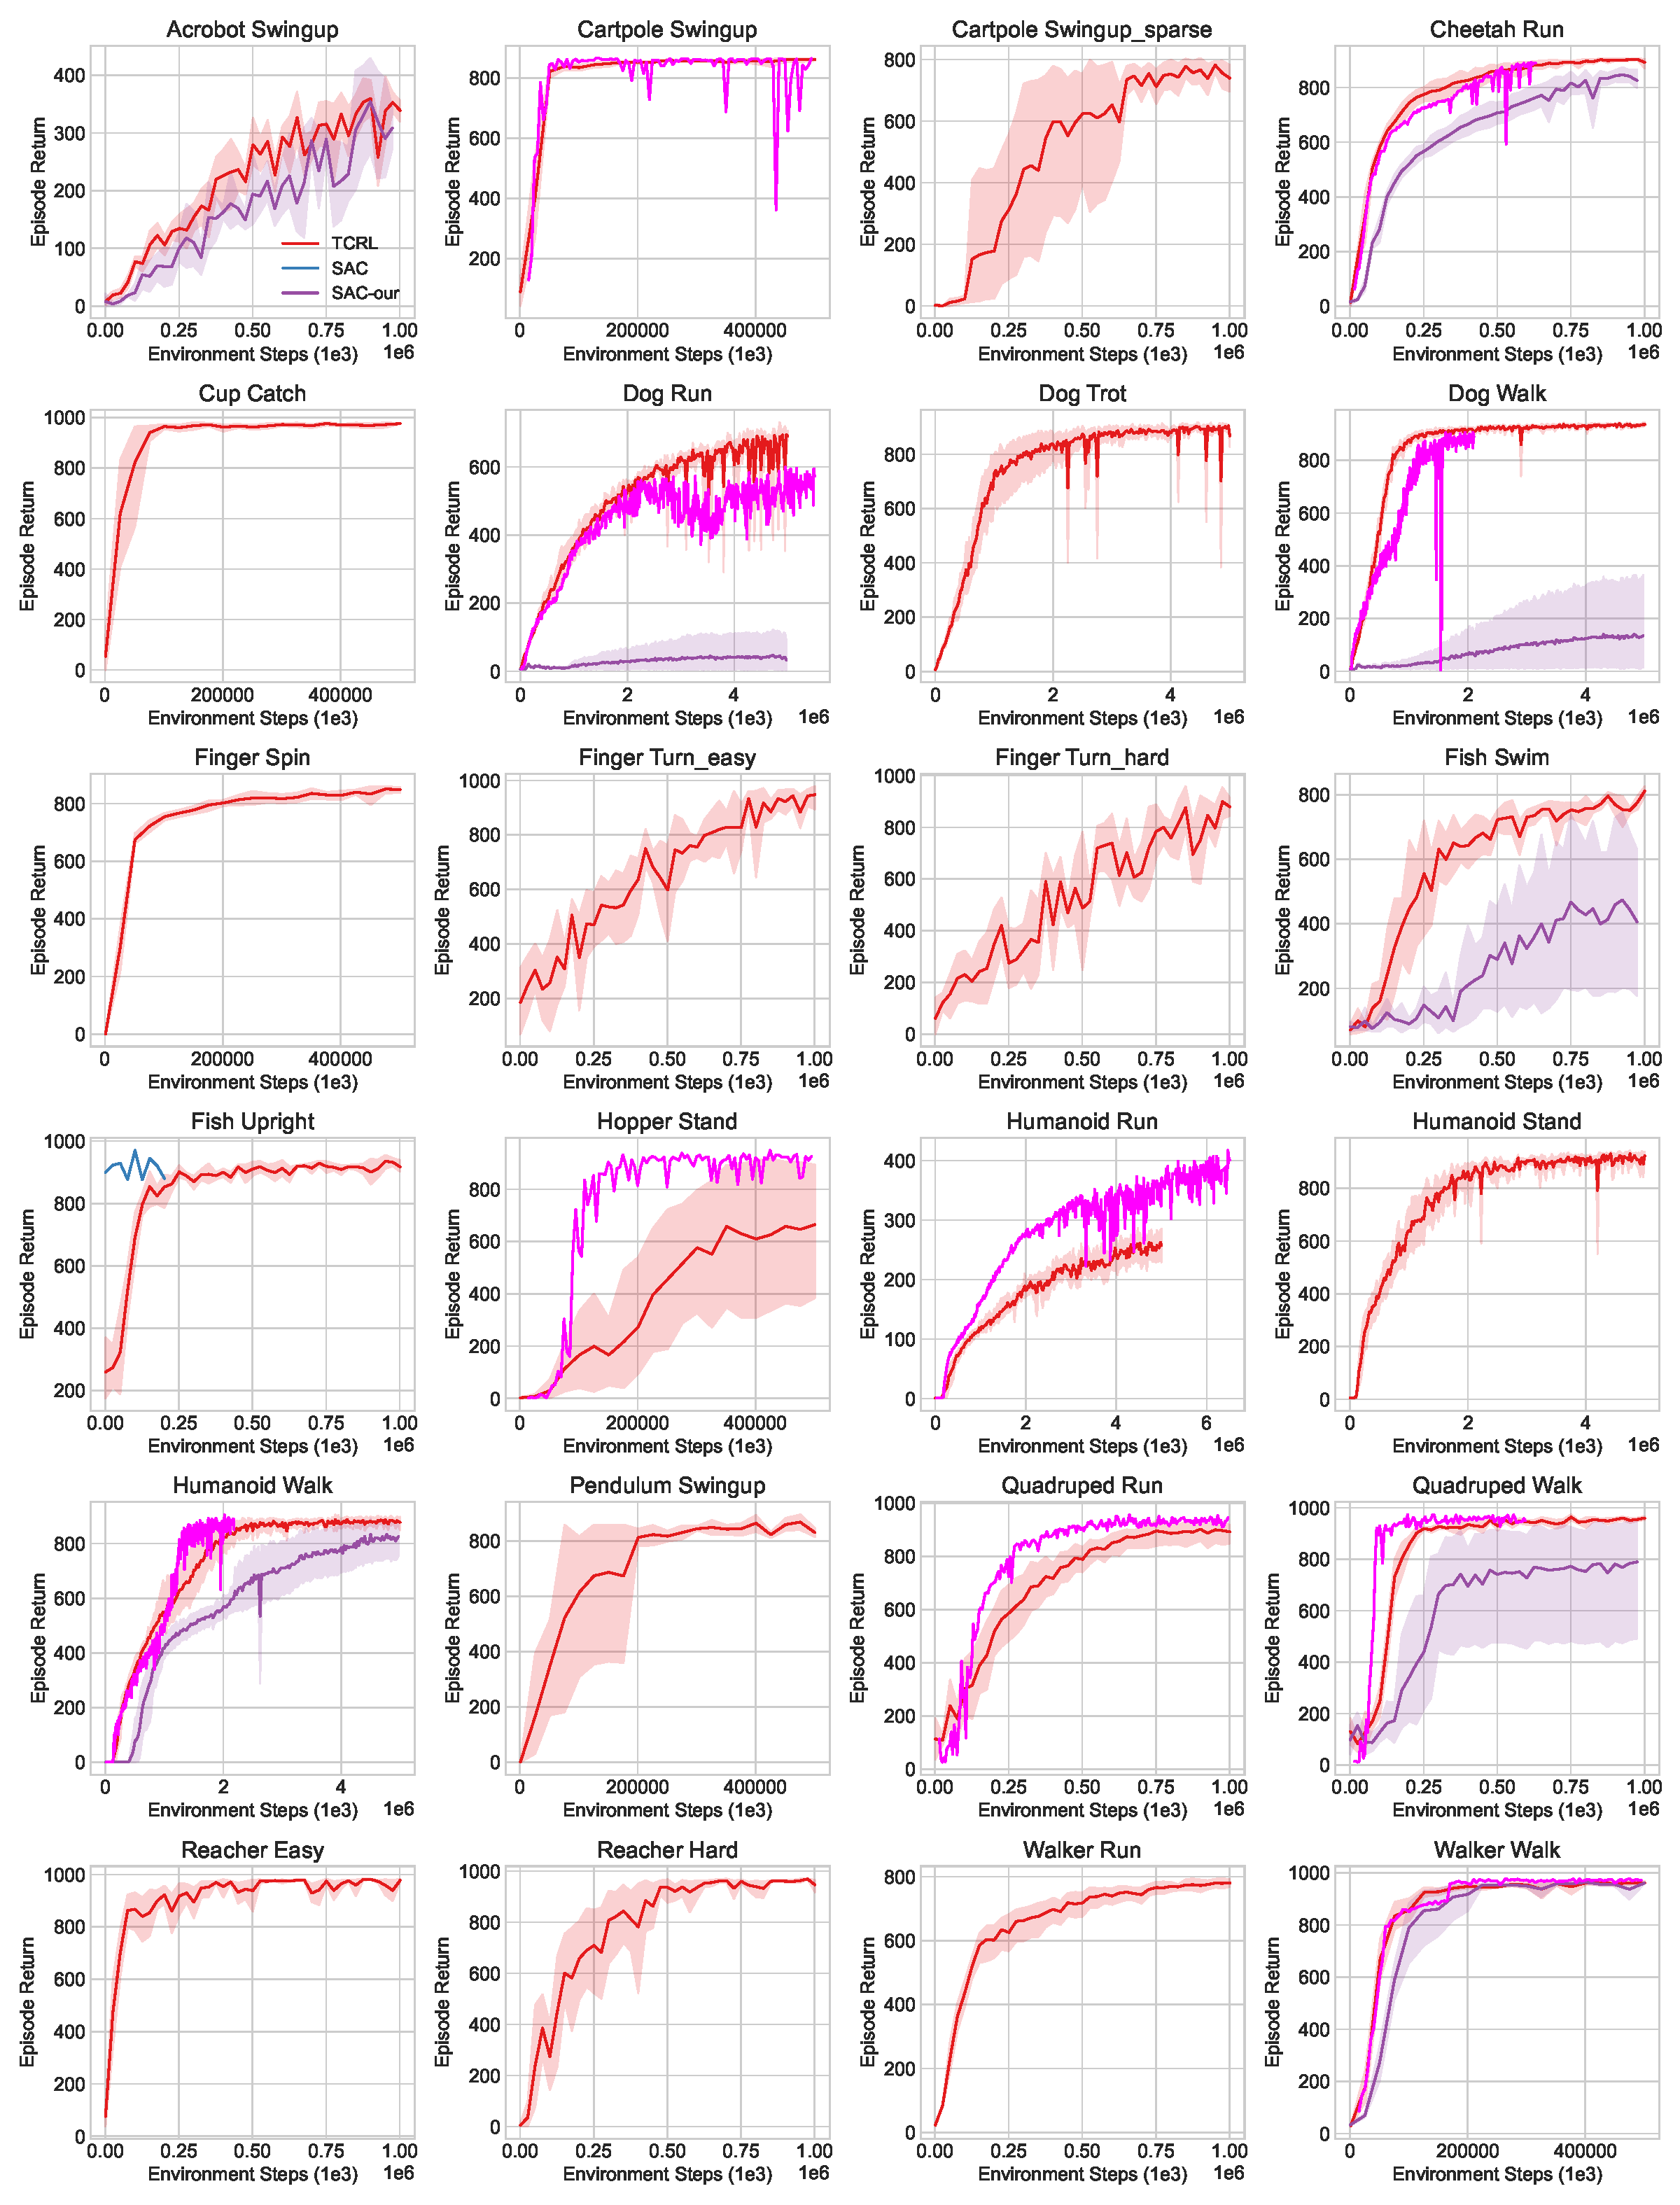
\includegraphics[width=0.97\textwidth]{./figs/all_mujoco_envs.pdf}}
% \caption{Comparison to SAC/TCRL with UTD=1.}
% \label{fig:main_plot}
% \end{center}
% \vskip -0.2in
% \end{figure*}


%%%%%%%%%%%%%%%%%%%%%%%%%%%%%%%%%%%%%%%%%%%%%%%%%%%%%%%%%%%%%%%%%%%%%%%%%%%%%%%
%%%%%%%%%%%%%%%%%%%%%%%%%%%%%%%%%%%%%%%%%%%%%%%%%%%%%%%%%%%%%%%%%%%%%%%%%%%%%%%



\end{document}


% This document was modified from the file originally made available by
% Pat Langley and Andrea Danyluk for ICML-2K. This version was created
% by Iain Murray in 2018, and modified by Alexandre Bouchard in
% 2019 and 2021 and by Csaba Szepesvari, Gang Niu and Sivan Sabato in 2022.
% Modified again in 2023 and 2024 by Sivan Sabato and Jonathan Scarlett.
% Previous contributors include Dan Roy, Lise Getoor and Tobias
% Scheffer, which was slightly modified from the 2010 version by
% Thorsten Joachims & Johannes Fuernkranz, slightly modified from the
% 2009 version by Kiri Wagstaff and Sam Roweis's 2008 version, which is
% slightly modified from Prasad Tadepalli's 2007 version which is a
% lightly changed version of the previous year's version by Andrew
% Moore, which was in turn edited from those of Kristian Kersting and
% Codrina Lauth. Alex Smola contributed to the algorithmic style files.
